\section{The strong force}

Question: What holds the nucleons (protons/neutrons) in a nucleus together?

\subsection{The early days: the Yukawa particle}

Based on the fact that the force holding nucleons together must be short range, as nucleons can be observed as free particles, without necessarily bonding into a nucleus, Hideki Yukawa in the 1930's (before the advent of Quantum Chromodynamics-QCD) suggested that the force holding nucleons together must be short range. {\bf Carrier of the strong force must be massive}, following the argument of Sec.~\ref{sec:massive_field}.

We can get an idea of what the mass of this force carrier should be by
considering that this carrier borrows some amount of energy $\Delta E$ (which is ok as long as it is paid back in time $\Delta t$ according to $\Delta E\Delta t\geq\hbar/2$) and traverses a distance $r_0$ determined by the size of a nucleon (the carrier needs to be exchanged between two nucleons in a nucleus).

We therefore have 
\[\Delta E\Delta t\sim\hbar/2,\]
\[\Delta t \sim\frac{r_0}{c},\] 
and \[\Delta E\sim m_{c}c^2.\]
Therefore for a nucleon size of $r_0\sim 10^{-15}$~m we can solve for $m_c$
yielding \[m_c=\frac{\hbar}{2r_0c}\sim 200m_e\sim \frac{1}{10}m_p\sim100~{\rm MeV}\]\footnote{This is just a dimensionality argument as you can see we have assumed a massive object travels at the speed of light...}
The fact that the mass of this carrier ($m_c$) is between the mass of a proton and the mass of the electron, it was named a meson (meaning in between).

\subsection{Discovery of the Yukawa meson}
\begin{figure}
\caption{Cecil Frank Powell}
\begin{tabular}{cc}
\parbox{0.32\textwidth}{
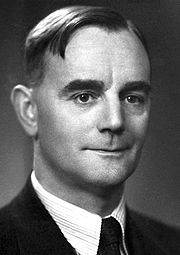
\includegraphics[width=0.3\textwidth]{fig/strongforce/180px-Cecil_Powell.jpg}
}&
\parbox{0.66\textwidth}{\textsf{\small
    ``Cecil Frank Powell took up a post in 1928 as Research Assistant to A.M. Tyndall in the H.H. Wills Physical Laboratory at the University of Bristol, later being appointed lecturer, and in 1948 appointed Melville Wills Professor of Physics. He was awarded the Nobel Prize in Physics for his development of the photographic method of studying nuclear processes and for the resulting discovery of the pion.'' 
}}
\end{tabular}
\\  \textsf{Source: \httplink{https://en.wikipedia.org/wiki/C.\_F.\_Powell}}
\end{figure}

In 1947 our very own Cecil Powell discovered a particle with a mass compatible to the mass of the Yukawa meson by measuring the traces that cosmic rays left in emulsion films on tops of mountains and air balloons. This Yukawa meson was called the Pion! He was awarded the Nobel Prize in 1969 for this discovery and the development of the photographic method for studying nuclear processes.
The principle of emulsion detection is very similar to that of a photographic film, offering high position resolution. A charged particle passing through the emulsion ionises atomic electrons of the emulsion. These electrons get trapped at a lattice defect at the surface of a crystal which makes up the emulsion. The trapped electrons in turn cause a chemical reaction which results in the development of (silver) filaments which manifest themselves as a dark spot on the emulsion.
\begin{figure}[!h]
\label{fig:pion_emulsion}
\begin{center}
\caption{Pion track captured in a photographic emulsion exposed to cosmic radiation. Pion enters the emulsion plate on the left of the image (track A) and undergoes multiple small angle scatters, loosing energy until it is captured by a nucleus which then disintegrates into proton tracks B,C,D. The top figure is a picture of the actual emulsion plate. The bottom figure is a trace of the star-shaped tracks on the right hand side of the top image. \textsf{Source: Nature 159 (1947)}.}
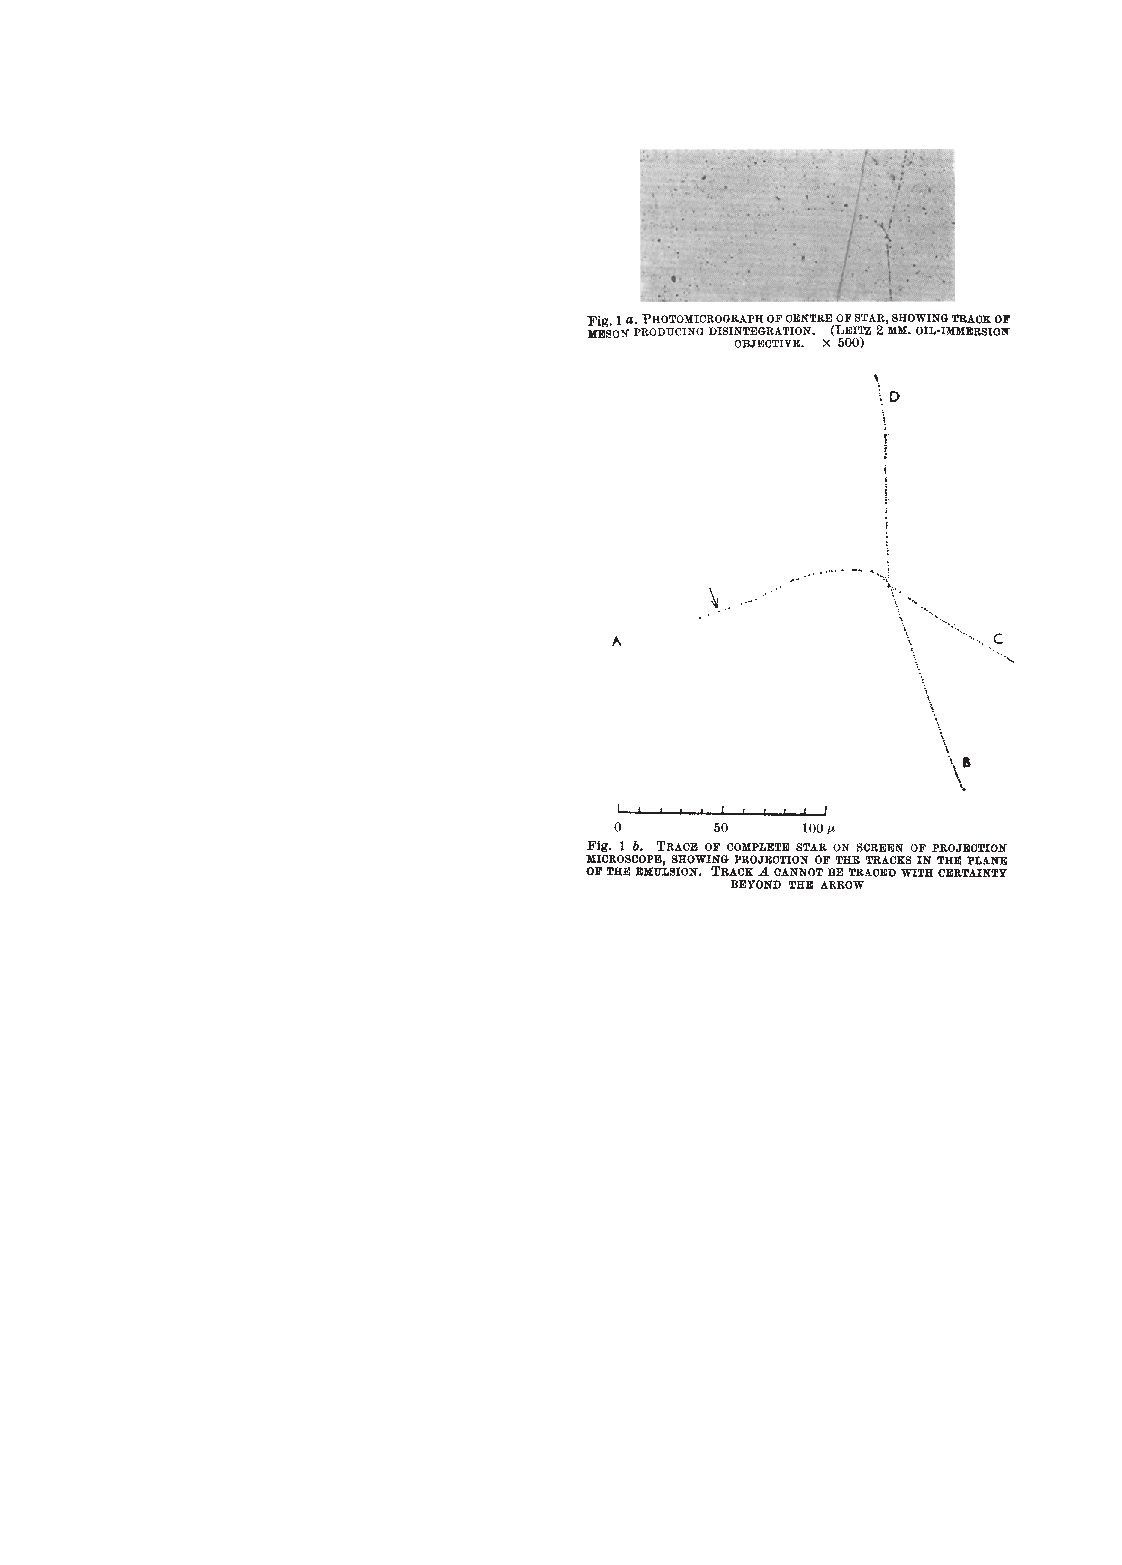
\includegraphics[width=0.80\textwidth]{fig/strongforce/pion_emulsion.pdf}
\end{center}
\end{figure}
By measuring the density of dots the pion left in the emulsion, as shown in Fig.~\ref{fig:pion_emulsion}, the angles at which the pion track scattered as it travelled through the emulsion, and the range the pion travelled before decaying, Powell was able to show that the mass of the pion was compatible to the mass of the Yukawa meson. In order to understand however how he could make such a measurement we need to understand how particles interact with matter.
\clearpage


\subsection{Consequences of the $\pi$-meson discovery}
\label{sec:isospinProtonsNeutronsPions}

\paragraph{It all made sense:} With the discovery of the pion it seemed that
strong interactions where completely understood. The nucleus is made up of proton and neutrons held together by a force mediated by the pion with a compling strength far larger ($\times 100$) in order to overcome the charge repulsion betwen the protons and hold the nucleus together.

Various scattering experiments between $p$ and $n$ as well as the binding energy of deuteron revealed that:
\begin{enumerate}
\item $m_p\sim m_n$
\item elastic scattering of protons and neutrons such as: 
\begin{center}
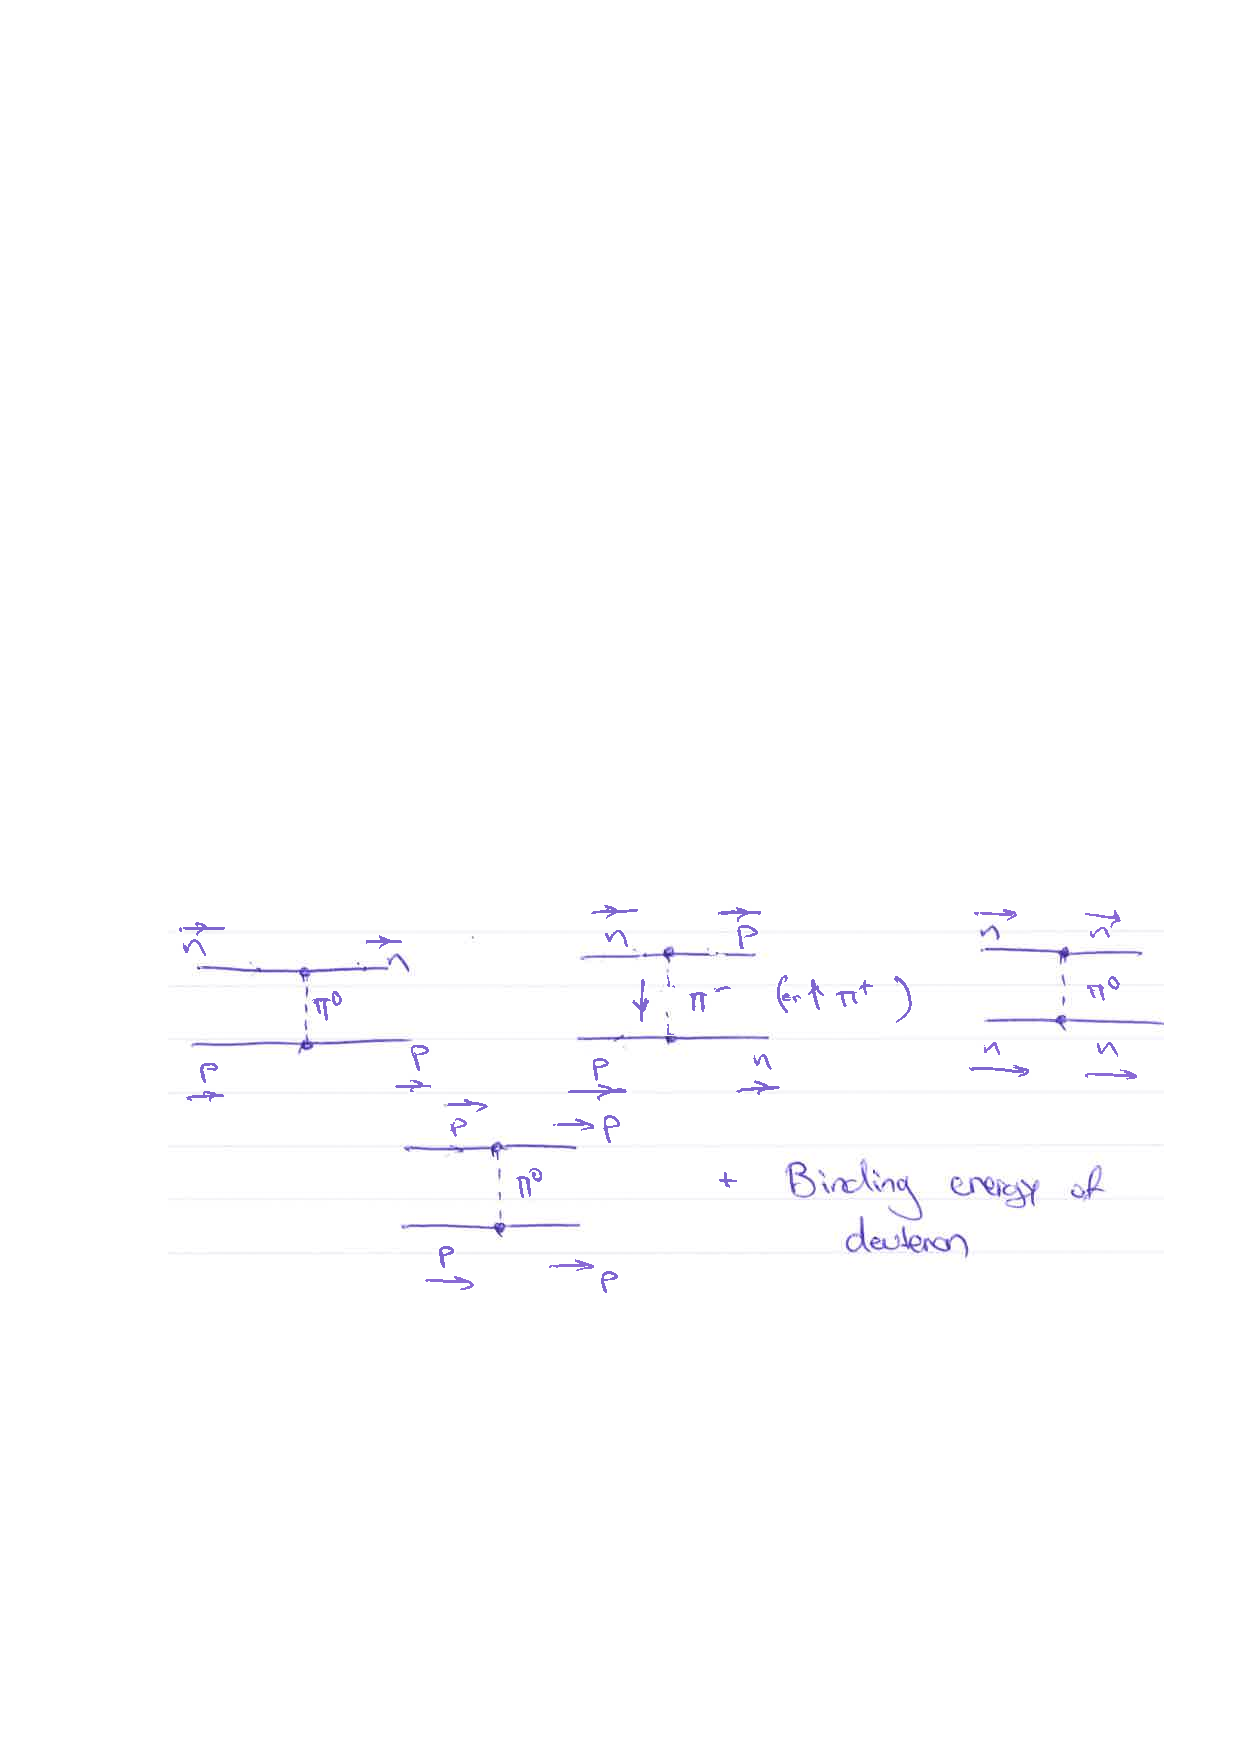
\includegraphics[width=0.98\textwidth]{fig/strongforce/proton_neutron_scattering.pdf}
\end{center}
all have same coupling strengths and must therefore have 3 different $\pi$-meson mediators with charges $0$, $+$ and $-$.
\end{enumerate}
The above two points means that the Strong force acts the same if in a process involving neutrons and or protons, you swap the neutrons with protons and vice versa.

Heisenberg in 1932 suggested that the neutron and the proton are considered as different states of a single entity ``the Nucleon'', in complete analogy to an electron which has two spin states: spin-up and spin-down. He therefore called this new quantum number Strong-Isospin.

For $n$ and $p$ which form an Isospin-Doublet: $I_s=\frac{1}{2}$ with $I_{s3}=\pm\frac{1}{2}$. Conventionally $I_{s3}^{p}=+\frac{1}{2}$ and $I_{s3}^{n}=-\frac{1}{2}$. 

Similarly, $\pi^+$, $\pi^-$ and $\pi^0$ mesons form an Isospin-Triplet with 
$I_{s}=1$, $I_{s3}^{\pi^+}=+1$, $I_{s3}^{\pi^0}=0$, $I_{s3}^{\pi^-}=-1$.

Points 1 and 2 suggest that the strong isospin operator $\hat{I_s}$ commutes with the hamiltonian
of the strong interactions $\hat{H_{s}}$. This in turn means that strong isospin is conserved in strong interaction. This means that under a strong interaction, the strong isospin of an initial state must be the same as strong isospin of the final state. Lets take a look at some reactions:

\paragraph{Examples}: 
\begin{itemize}
\item Consider the process $pp\to d\pi^+$ where $d$ is a Deuteron. The deuteron carries $I_s=0$ and $I_{s3}=0$. Using Dirac notation to denote the strong isospin states ($|I_s,I_{s3}>$), the initial state is a combination of two $|1/2,1/2>$ states, ie
\[
{\rm Initial:}~|1/2,1/2>|1/2,1/2>=|1,1>\\
\]
In contrast the final state is a combination of a $|0,0>$ and $|1,1>$ states, ie
\[
{\rm Final:}~|0,0>|1,1>=|1,1>
\]

Note that we have used the principles of quantum mechanical angular momentum addition to determine the total isospin of the initial and final states. Remember: 
\[
|I_{s}^{(1)}-I_{s}^{(2)}|\leq I_{s}^{tot}\leq I_{s}^{(1)}+I_{s}^{(2)}
\]
\[
I_{s3}^{tot}=I_{s3}^{(1)}+I_{s3}^{(2)}
\]
So combining two $|1/2,1/2>$ states gives us $|1,1>$. In contrast, combining a $|0,0>$ with a $|1,1>$ state gives us a $|1,1>$ state. So in this process the total strong isospin of the initial and final states is the same and therefore the process conserves strong isospin and is therefore allowed.

\item Consider the process $pn\to d\pi^0$. The initial state is a combination of a $|1/2,1/2>$ and $|1/2,-1/2>$ states, ie
\[
{\rm Initial:}~|1/2,1/2>|1/2,-1/2>=\sqrt{\frac{1}{2}}(|1,0>+|0,0>).\\
\]
In contrast the final state is a combination of a $|0,0>$ and $|1,0>$ states, ie
\[
{\rm Final:}~|0,0>|1,0>=|1,0>
\]
Note that we have again used the principles of quantum mechanical angular momentum addition
to determine the total isospin of the initial and final states.

We also make use of the Clebsch-Gordan coefficients to determine the exact mixture
of total isospin states. Don't worry if you have never seen this. We will give
you the expressions for the total isospin states anyway. Lets explain a bit in detail how we reached this result:

So combining  states $|1/2,1/2>$ and $|1/2,-1/2>$, 
results in $I_{s}^{tot}=0$ or $I_{s}^{tot}=1$ with $I_{s3}^{tot}=0$. The Clebsh-Gordan table tells us that we can therefore write: $|1/2,1/2>|1/2,-1/2>=\sqrt{\frac{1}{2}}(|1,0>+|0,0>)$.

However combining states $|0,0>|1,0>$ results in only one option, $I_{s}^{tot}=1$ with $I_{s3}^{tot}=0$.

Ok so how does strong isospin conservation fit into all this? Well the final state is $|1,0>$, therefore since isospin is conserved, only $pn$ states in a $|1,0>$ and NOT in a $|0,0>$ can decay to a $d\pi^0$ state. This means that in contrast to the previous example, where both initial and final states are found in a single configuration, the process $pn\to d\pi^0$ occurs at a lower rate by a factor of $\sqrt{\frac{1}{2}}^2=\frac{1}{2}$ compared to $pp\to d\pi^+$.
This is because the initial $pn$ state must be in a $|1,0>$ in order to decay via the strong interaction to $d\pi^0$ which is also a $|1,0>$ state. The probability of the $pn$ state to be in a $|1,0>$ configuration is given by the square of the coefficient in front of the $|1,0>$ term ie
$\sqrt{\frac{1}{2}}^2$.
\item The $\rho^0$ meson is an excited state of the $\pi^0$ meson. It has a strong isospin state of $|1,0>$. The $\rho^0$ decays primarily to a $\pi^+$ and a $\pi^-$ but never to a pair of $\pi^0$ mesons. One of the reasons is because the decay of the $\rho^0$ primarily occurs through the strong force so isospin must be conserved. Lets consider the isospin configurations of the two final states (consulting the Clebcsh-Gordan table):
\[
\pi^0\pi^0: |1,0>|1,0> =\sqrt{\frac{2}{3}}|2,0>+0|1,0>-\sqrt{\frac{1}{3}}|0,0>
\]
\[
\pi^+\pi^-: |1,1>|1,-1> =\sqrt{\frac{1}{6}}|2,0>+\sqrt{\frac{1}{2}}|1,0>+\sqrt{\frac{1}{3}}|0,0>
\]
Therefore as you can see the factor in front of the $|1,0>$ state which corresponds to the strong isospin state of the $\rho^0$ is 0! This means that 2 $\pi^0$ mesons can never be in a strong isospin configuration required by the $\rho^0$, in contrast to the $\pi^+\pi^-$ state which can. This means that the $\rho^0$ CAN decay via the strong force to $\pi^+\pi^-$ but CANNOT decay to  $\pi^0\pi^0$\footnote{You will see later that $\rho^0\to\pi^0\pi^0$ also violates another symmetry of both the strong and electromagnetic interactions: Charge-conjugation symmetry.}.

\end{itemize}

\subsection{Extending Strong-Isospin to the quark sector and the existence of colour}
\label{sec:isospinQuarks}
The proton is made up of 2 up-type quarks and 1 down-type quark (uud).
The neutron is made up of 1 up-type quark and 2 down-type quarks (udd).
We can extend the idea that the strong force treats neutrons and protons equally,
to treating up-type and down-type quarks equally. 

So as we did before, we consider the up and down quarks as different states of a single
entity. The strong isospin of the up-quark has $I_{s}=\frac{1}{2}$ with 
$I_{s3}=+\frac{1}{2}$ and the down-quark has $I_{s}=\frac{1}{2}$ with $I_{s3}=-\frac{1}{2}$.
We can therefore use the principles behind angular momentum addition, to construct the total isospin of the proton, neutron and other quark bound states. 

So combining three quarks of two isospin states (or quark flavours $u=|\frac{1}{2},+\frac{1}{2}>$ and $d=|\frac{1}{2},-\frac{1}{2}>$) we get
eight states: $uuu,~uud,~udu,~udd,~duu,~dud,~ddu,~ddd$ with total isospin:
\begin{center}
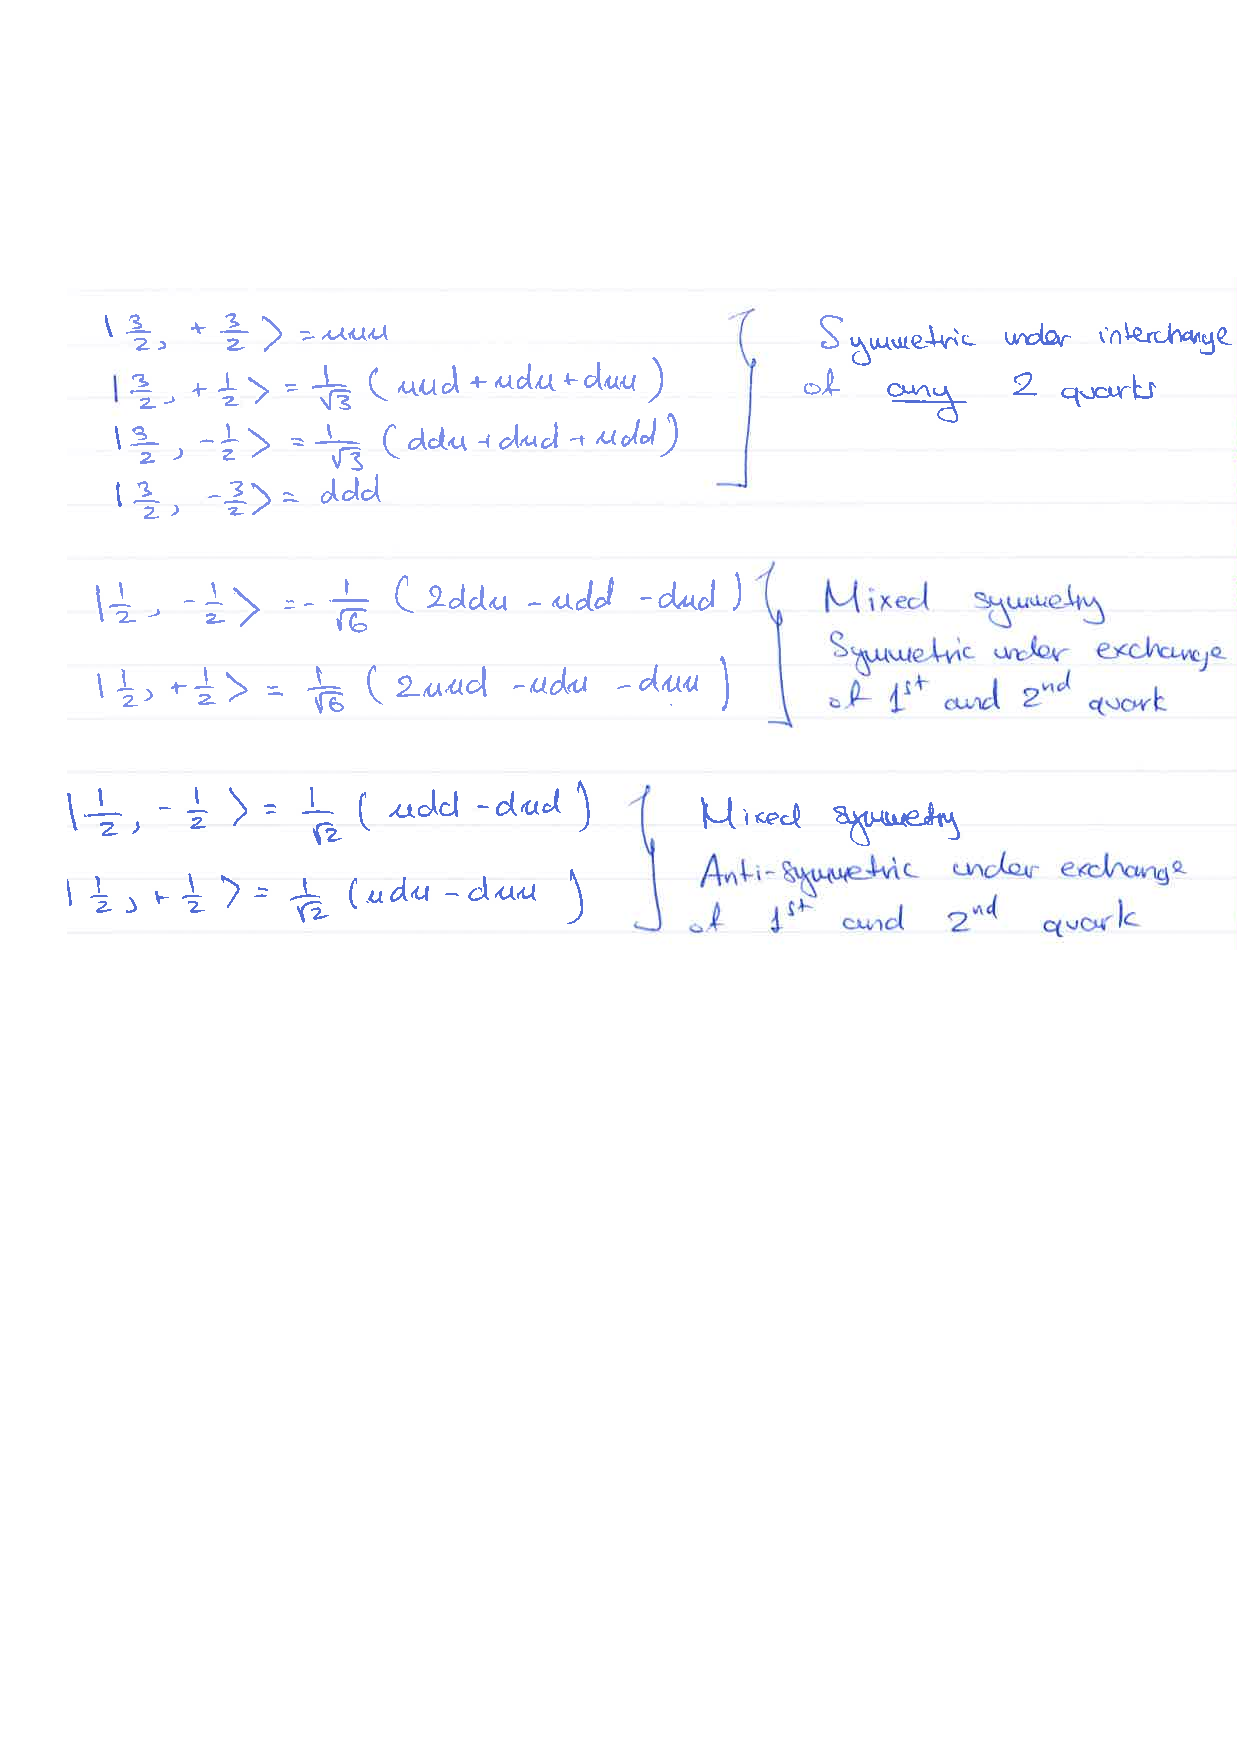
\includegraphics[width=0.98\textwidth]{fig/strongforce/baryon_isospin.pdf}
\end{center}
Ok so why stop here. Lets play the same game with the spin of this three-quark system. Remember quarks are fermions, they obey the Dirac equation and therefore carry spin $S=\frac{1}{2}$ and $S_3=\pm\frac{1}{2}$. So just like with isospin, we have eight spin states:
\begin{center}
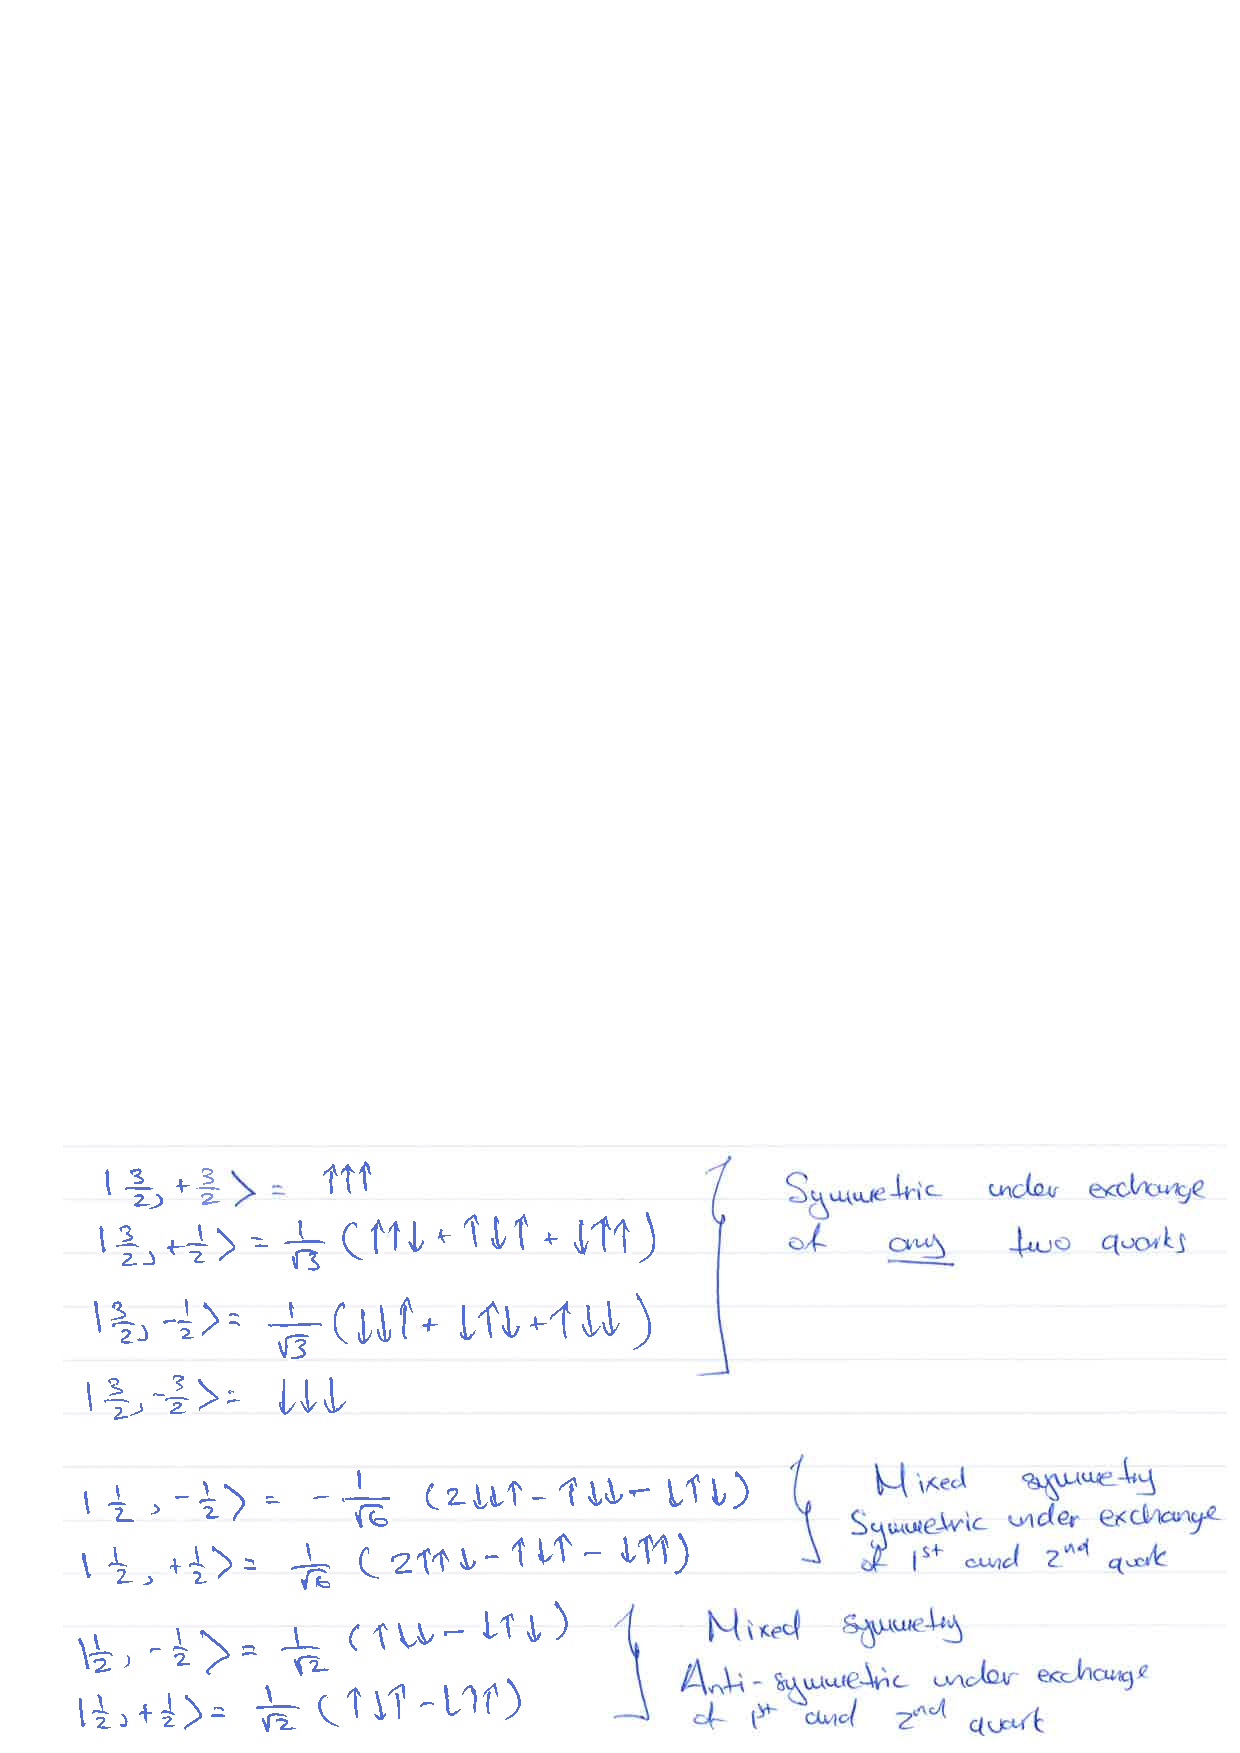
\includegraphics[width=0.98\textwidth]{fig/strongforce/baryon_spin.pdf}
\end{center}

So far we have considered two parts of the total wave-function of a bound state of 3 quarks (known as a Baryon). There is an additional part of the wave-function relating to the spatial part of the 3-quark combination. Putting all this together we have
\begin{equation}
\label{eq:psi_total_no_colour}
\psi_{\rm total}=\phi_{\rm isospin}\chi_{\rm spin}\eta_{\rm space}.
\end{equation}

Now given that baryons are made of up 3 quarks (fermions) there is another aspect we need to consider. The Pauli exclusion principle states that no two electrons (also fermions) can occupy the same quantum number state. This principle was devised in order to be able to explain why atomic electrons don't all cascade down to the ground state. This might sound somewhat ad-hoc however the Pauli principle is rooted on something deeper. 

{\bf The wave function of indistinguishable fermions must be anti-symmetric under the exchange of any two fermions.}
This means that for a wave function made up of two particles $\psi(1,2)$, must satisfy $\psi(1,2)=-\psi(2,1)$.

For example, consider one fermion in state $\psi_\alpha$ and a second fermion in state $\psi_\beta$. The total wave function is $\psi(1,2)=\psi_\alpha(1)\psi_\beta(2)$.
However, since the fermions are indistinguishable, the state  $\psi(1,2)=\psi_\alpha(2)\psi_\beta(1)$ is indistinguishable from the previous one. Thus both of these
wavefunctions describe the same state so we need to take the superposition of them. Since we require that $\psi(1,2)=-\psi(2,1)$, we can write $\psi(1,2)$ as
\footnote{Similarly, indistinguishable bosons would satisfy
$\psi(1,2)=\frac{1}{\sqrt{2}}[ \psi_\alpha(1)\psi_\beta(2)+\psi_\alpha(2)\psi_\beta(1)]$.
}
\[
\psi(1,2)=\frac{1}{\sqrt{2}}[ \psi_\alpha(1)\psi_\beta(2)-\psi_\alpha(2)\psi_\beta(1) ].
\]
We can now see Pauli's exclusion principle in action. If both fermions $1$ and $2$ where in the same state $\alpha$, then  $\psi(1,2)=0$.

Coming back to Eq.~\ref{eq:psi_total_no_colour}, from what we have learnt, $\psi_{\rm total}$ of the baryon must be antisymmetric under the exchange of any pair of quarks. For what follows let us consider only ground state baryons, that is baryons withe orbital angular momentum $L=0$. In this case, $\eta_{\space}$ is totally symmetric. This means that the product $\phi_{\rm isospin}\chi_{\rm spin}$ must be totally anti-symmetric. This in turn would mean that the state
\[
(uuu)(\uparrow\uparrow\uparrow)=|(\frac{3}{2},+\frac{3}{2})_{\rm isospin},(\frac{3}{2},+\frac{3}{2})_{\rm spin}>
\]
should not be a physical state as it is totally-symmetric. However in scattering
experiments of a $\pion$ beam off a proton target, a charge +2 particle was observed, the $\Delta^{++}$ compatible with a $(uuu)(\uparrow\uparrow\uparrow)$ state.



{\bf Therefore something is missing in Eq.~\ref{eq:psi_total_no_colour}. The missing ingredient is colour charge!}

In order to explain the observed pattern of baryons, their masses and spins another component to the wave-function of the baryon was required. The colour wave-function. Equation~\ref{eq:psi_total_no_colour} is then modified to
\begin{equation}
\label{eq:psi_total_colour}
\psi_{\rm total}=\phi_{\rm isospin}\chi_{\rm spin}\eta_{\rm space}\zeta_{\rm colour}.
\end{equation}
where $\zeta_{\rm colour}$ is antisymmetric under the exchange of any 2 quarks. 
The only completely anti-symmetric state has a net colour quantum number of 0.
{\bf All baryons and mesons have a net colour charge of 0}. 
So with our friend the $\Delta^{++}$, the requirement that $\zeta_{\rm colour}$ is totally antisymmetric, means that $\phi_{\rm isospin}\chi_{\rm spin}$ must be totally symmetric for ground state baryons.

\paragraph{Mesons:} Note that so far our focus has been on three quark bound states (baryons). We can follow a similar treatment of bound states of a quark and anti-quark (mesons) like the $\pi^+$ which is a $u\bar{d}$ state. Constructing the meson wave-function does not suffer from the complication that the overall wavefunction has to be anti-symmetric as we are dealing with distinguishable fermion anti-fermion states.

\paragraph{The strange quark:}
The discovery of strange hadrons (hadrons containing strange quarks) in cosmic rays such as the $K^+$ meson (a bound state between $u\bar{s}$) requires to add to the previous picture a new quantum number called strangeness. Strangeness is conserved in strong interactions but not in weak interactions. This is because the strange quark can decay to another quark through the weak interaction, as you will see later in the course. We know that the mass of the strange quark is not the same as the mass of the $u$ and $d$ quarks, however the mass 
difference between baryons that contain a strange quark is small compared to the total baryon mass. For example the $\Lambda^{0} (uds)$ has a mass of 1.1~GeV and the $n(udd)$  has a mass of 0.9~GeV. We can therefore say that the strong force is approximately symmetric under the exchange of a $u$ or $d$ quark, with an $s$ quark. We can refer to this symmetry as ``Flavour Symmetry''.
So we can repeat the above exercise where we extend strong-isospin of quarks to include the strange quark, that is we identify
$u=|1,+1>,s=|1,0>,d=|1,-1>$. 

\paragraph{Putting it all together:}
The plethora of hadronic states discovered during the 40s 50s and 60s could be explained using the principles of flavour symmetry, fermi-statistics and a new quantum number ``colour''. Murray Gell-Mann constructed this model in 1961 which led to the development of the quark model. His model predicted the existence of a spin-3/2 $sss$ state with a mass near $1680$~MeV (the $\Omega^-$). A particle matching these properties was subsequently discovered in 1964 which earned Gell-Mann the Nobel Prize in 1969.

\begin{center}
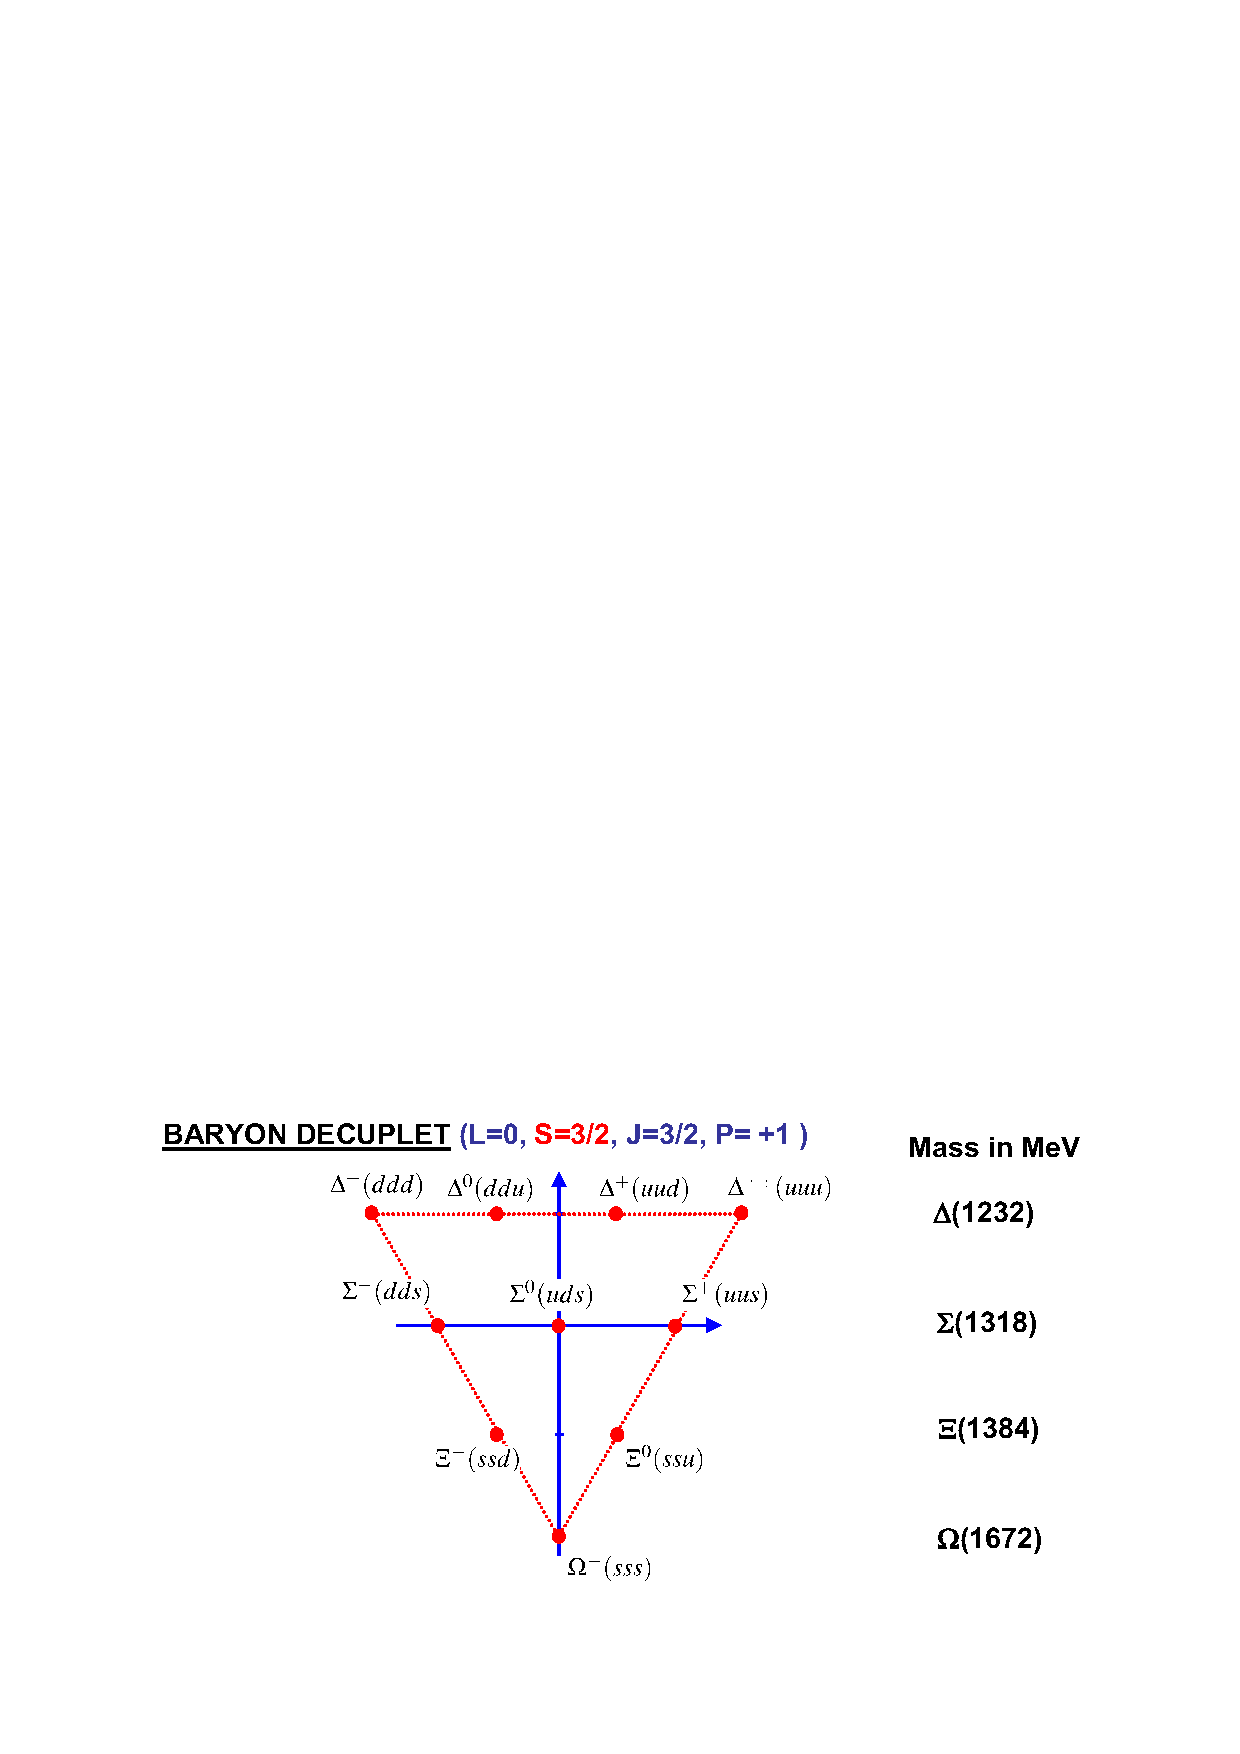
\includegraphics[width=0.65\textwidth]{fig/strongforce/baryon_decouplet.pdf}\\
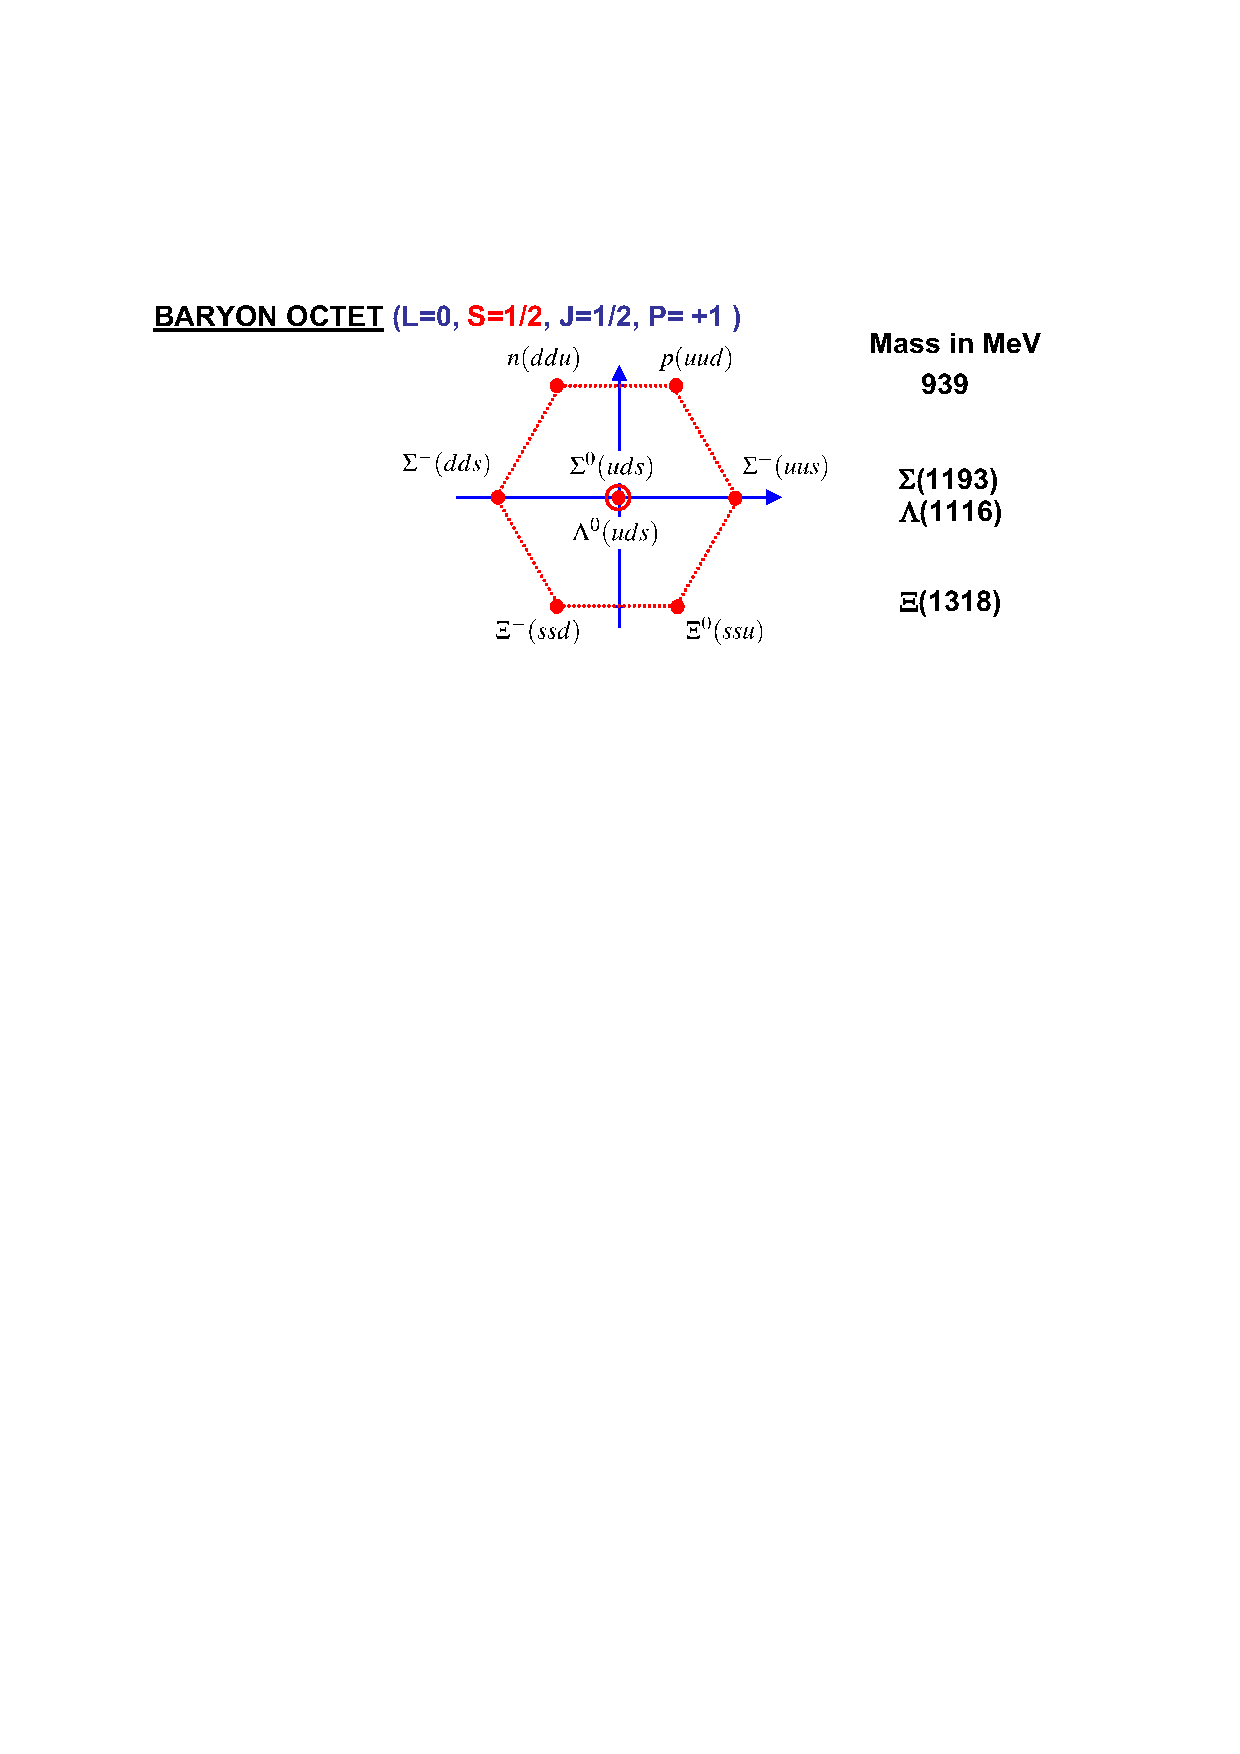
\includegraphics[width=0.7\textwidth]{fig/strongforce/baryon_octet.pdf}\\
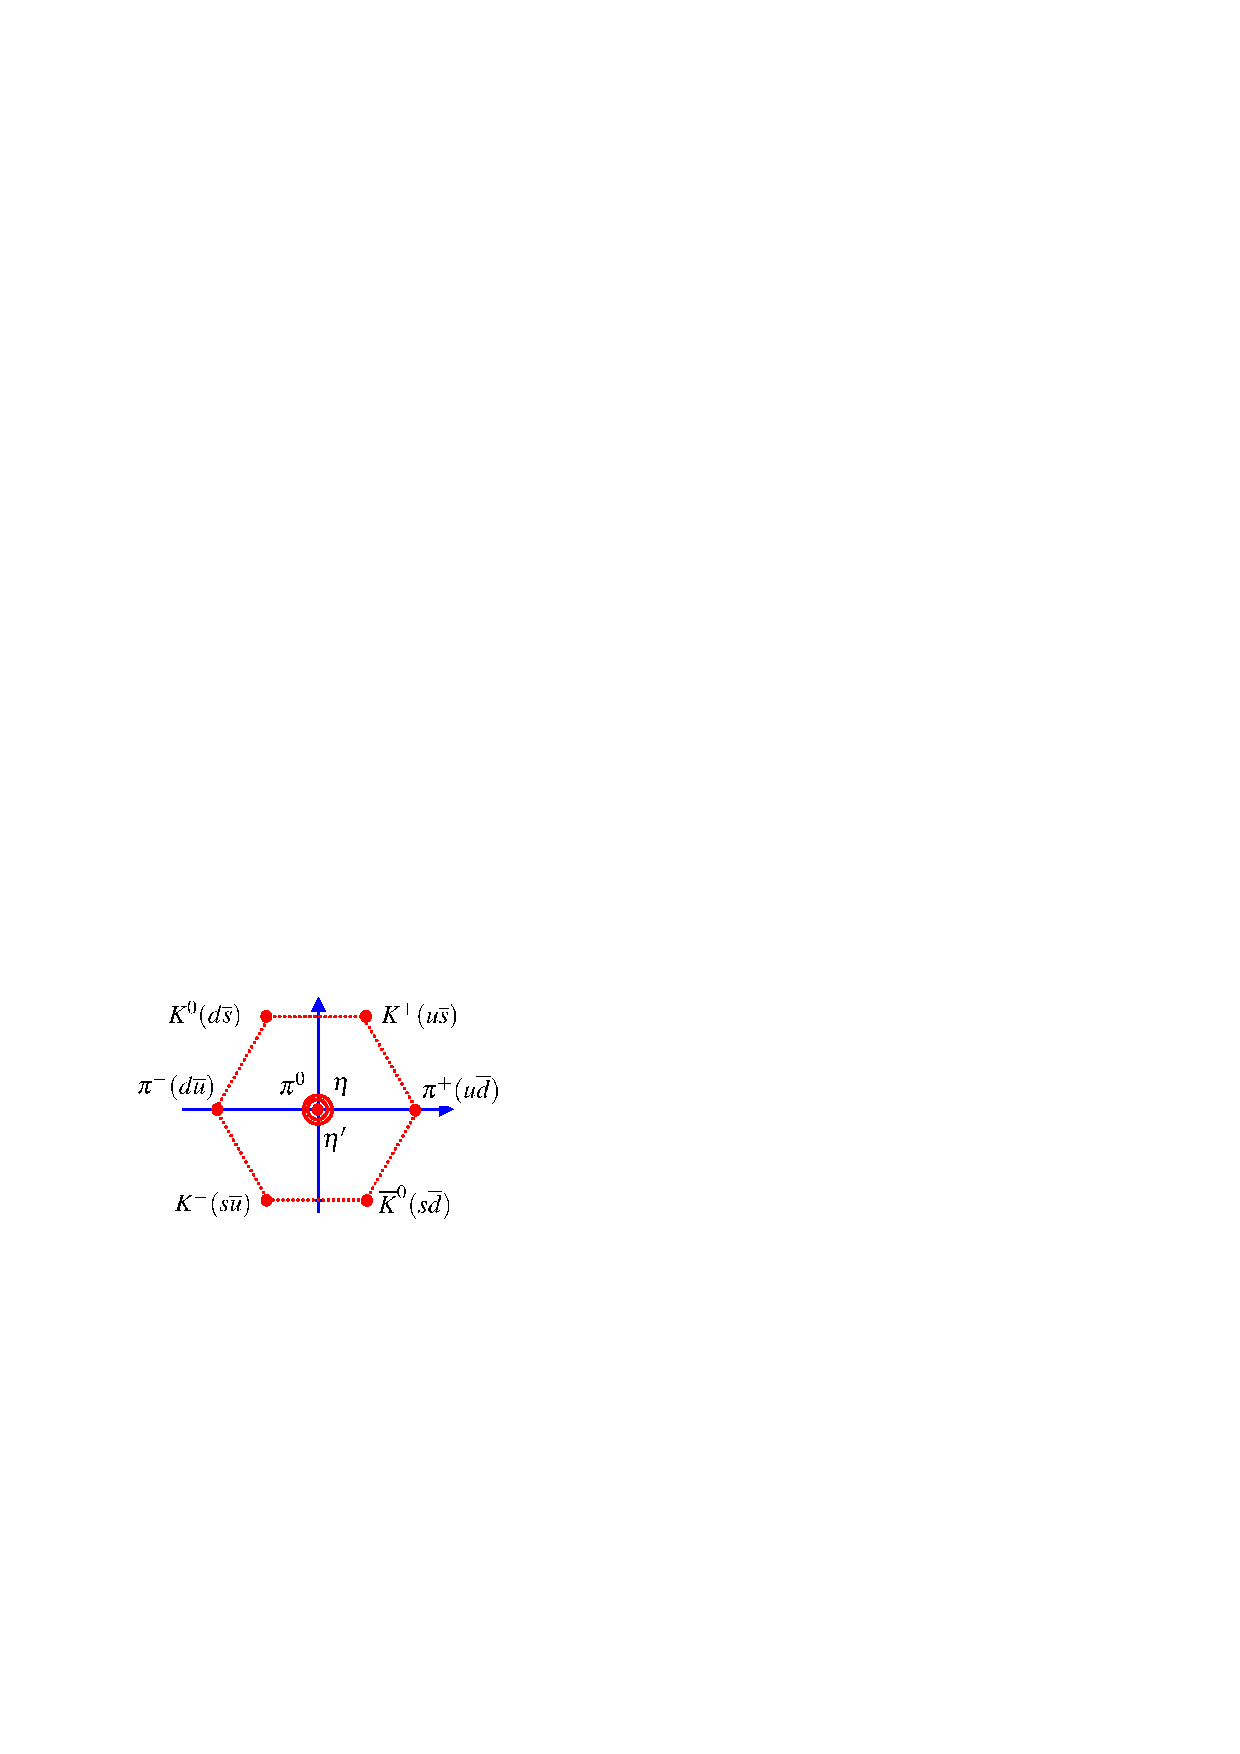
\includegraphics[width=0.4\textwidth]{fig/strongforce/scalar_mesons.pdf}\\
{\tiny Source: Prof. M. A. Thomson \httplink{http://www.hep.phy.cam.ac.uk/~thomson/lectures/partIIIparticles/Handout7\_2009.pdf}}
\end{center}
If flavour symmetry between the three quark types was exact, then all baryons and mesons would have exactly the same mass irrespective of how many strange quarks they contain.

\subsection{Colour Confinement}
We demonstrated that hadrons required an additional totally antisymmetric component to their wave-function. This was in order to explain the existence of the large number of observed baryons while still requiring that their overall wave-function is anti-symmetric under the exchange of any two quarks.

By requiring that each quark carries a new quantum number called ``colour'' (or ``colour charge'') we can construct a totally anti-symmetric wave function out of three quarks if the colour charge can have three values ``{\bf r}ed'', ``{\bf g}reen'', and ``{\bf b}lue''\footnote{You can see why you need three types of colour, because looking back at the symmetries of the spin part of the baryonic wave-function, you can see that you can never build a totally anti-symmetric wave function which is made up of 3 quarks and only two spin quantum numbers (spin-up, spin-down).}. Anti-quarks carry colour charges of ``anti-red'', ``anti-blue'', ``anti-green''.

In this case, there is a single such combination which also gives rise to a total colour charge of 0. For baryons this combination is:
\[
\zeta_{\rm colour}^{qqq}=\frac{1}{\sqrt{6}}(rgb-rbg+gbr-grb+brg-bgr)
\]
As discussed earlier, for mesons  there is no restriction that the wave function is antisymmetric as mesons are made up of distinguishable quarks and anti-quarks ($q\bar{q}$). However there seems to be a more fundamental principle that determines the colour wave-function of all hadrons and also restricts the types of bound states one could form out of quarks. This principle is known as ``colour confinement'', which states that:\\\\
{\bf Only states with a total colour charge of 0 can exist as free particles.}\\\\
There is no direct proof, other than all experimental evidence seems to point to this fact. This is the reason why the colour wave-function of mesons is given by:
\[
\zeta_{\rm colour}^{q\bar{q}}=\frac{1}{\sqrt{3}}(r\bar{r}+g\bar{g}+b\bar{b})
\]
which is has a total colour charge of 0. 

Additionally the above principle is also why we cannot form bound states of $qq\bar{q}$ or $qq$ quarks as we cannot obtain a colour-less state from these combination of quarks. However states like $q\bar{q}q\bar{q}$ and $qqqq\bar{q}$ are indeed allowed and the LHCb experiment (last July) seems to have some first hard evidence of the existence of such exotic states, as shown in Fig.~\ref{fig:lhcb_pentaquark}.
\begin{figure}
\centering
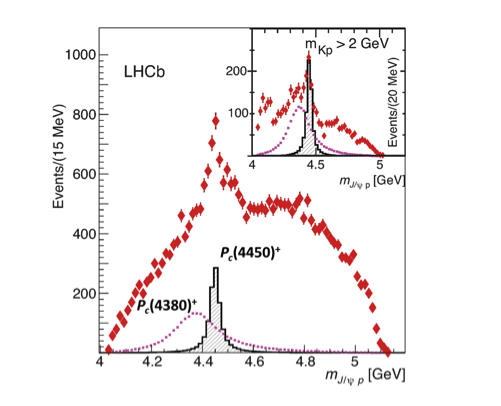
\includegraphics[width=0.65\textwidth]{fig/strongforce/lhcb_pentaquark.png}
\caption{The invariant mass between the proton ($p$) and the $J/\psi$ meson (a bound state of $c\bar{c}$ quarks) from the decay of a $\Lambda_{b}$ baryon (like a proton but with a $udb$ quark content) to a $J/\psi$, a proton and a $K^-$. The data are shown as red diamonds. The predicted distributions of the 5-quark bound states (penta-quarks) $P_c(4380)^+$ amd $P_c(4450)^+$ states are indicated in the purple and black distributions. The quark contents of these states are thought to be $uudc\bar{c}$.{\tiny Source:\httplink{http://press.web.cern.ch/press-releases/2015/07/cerns-lhcb-experiment-reports-observation-exotic-pentaquark-particles} and \httplink{http://arxiv.org/abs/1507.03414}}}
\label{fig:lhcb_pentaquark}
\end{figure}

\subsection{The role of the gluon in confinement}
Just like the EM charge, the strong charge is conserved at each vertex.
However, the fact that we have 3 types of colour charges for quarks, and 3 types
for anti-quarks means that the gluon, the massless carrier of the strong interaction, will also carry colour charge (in fact it carries one colour and one anti-colour charge). This is in contrast to EM interactions where the photon is electrically neutral.\footnote{For a formal proof of this effect take the 4th year course! If interested, it is because the gluon lies in the Lie algebra of an SU(3) group, compared to the photon which lies in the Lie algebra of a U(1) group}
\begin{center}
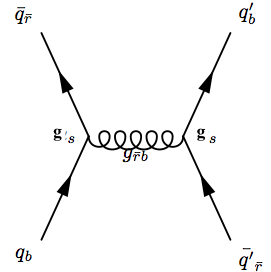
\includegraphics[width=0.5\textwidth]{fig/strongforce/gluon_qqbar.png}
\end{center}

The fact that the gluon now carries colour charge means that it can interact with itself so we have vertices of the type:
\begin{center}
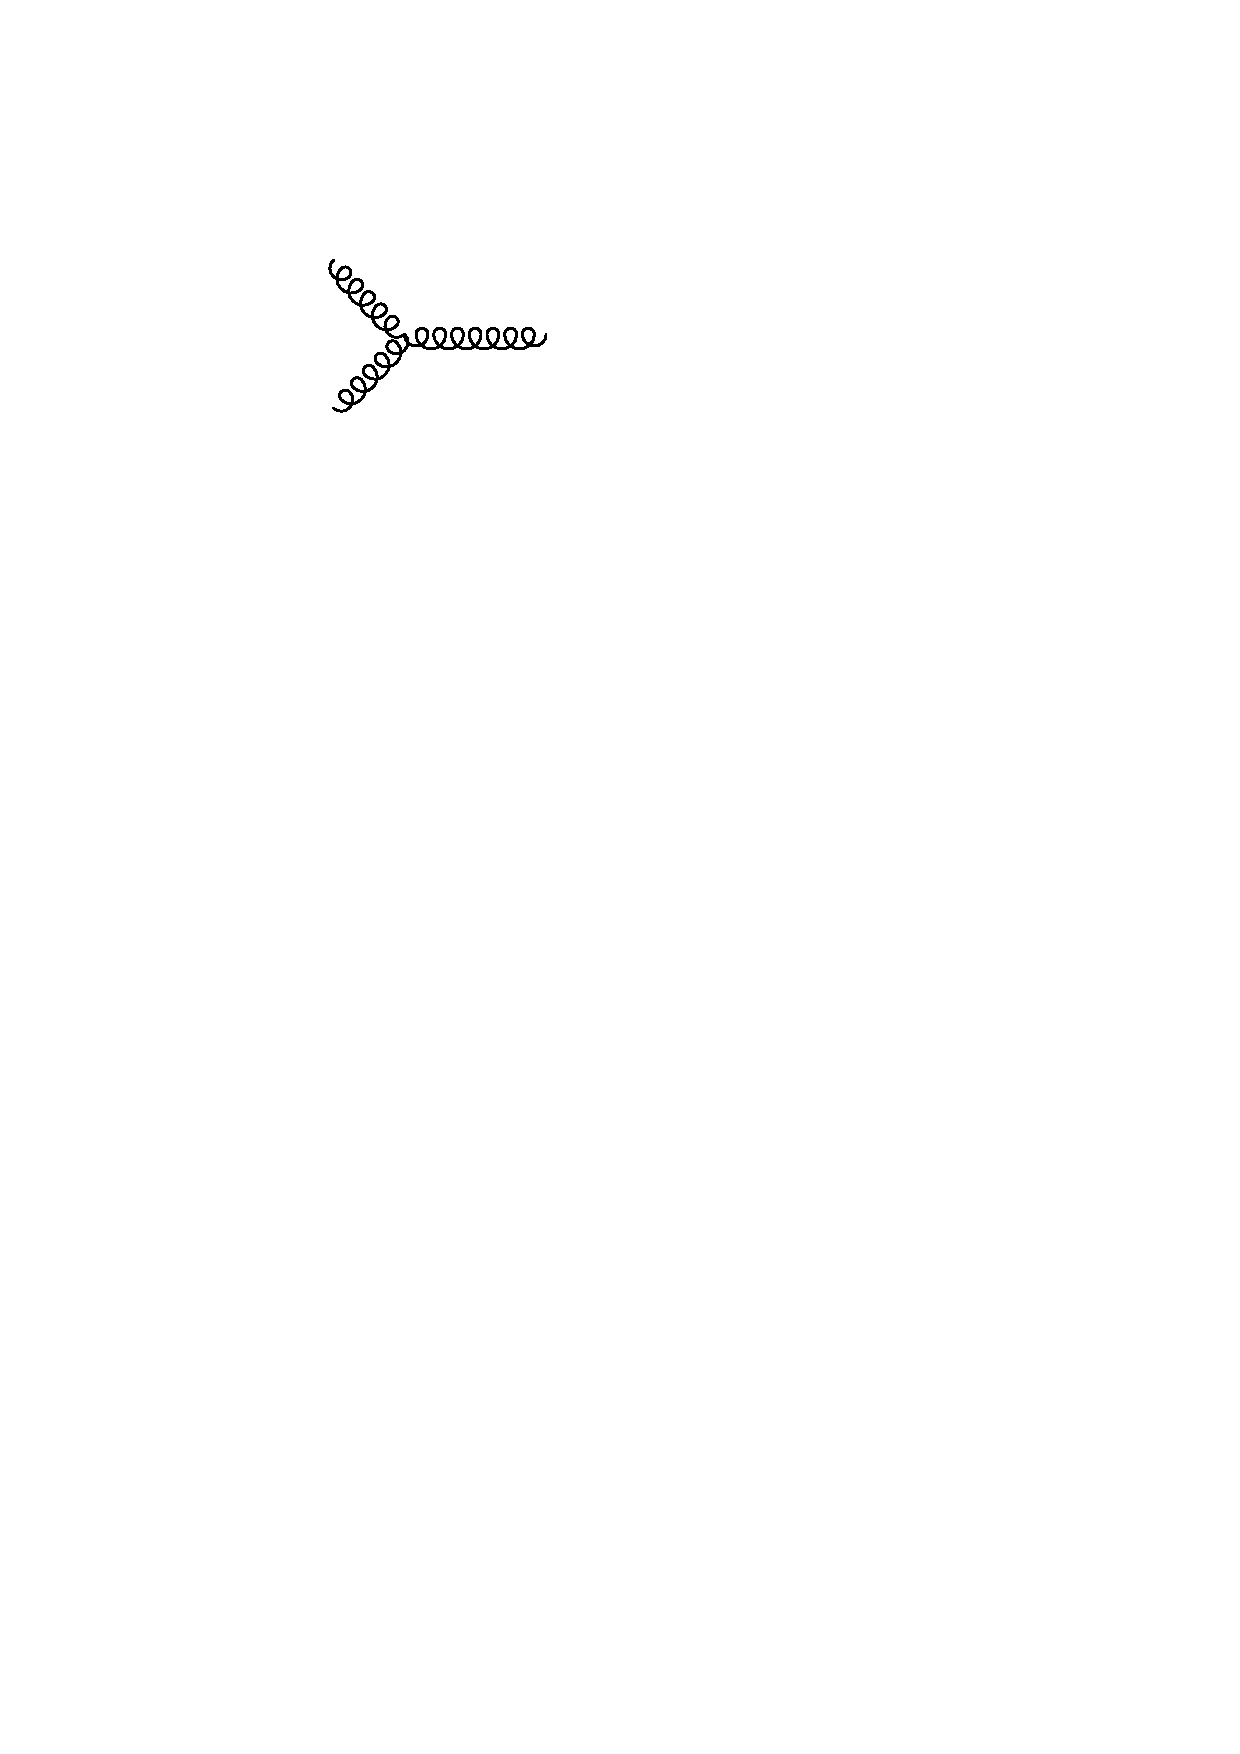
\includegraphics[width=0.3\textwidth]{fig/strongforce/gluon_three.pdf}
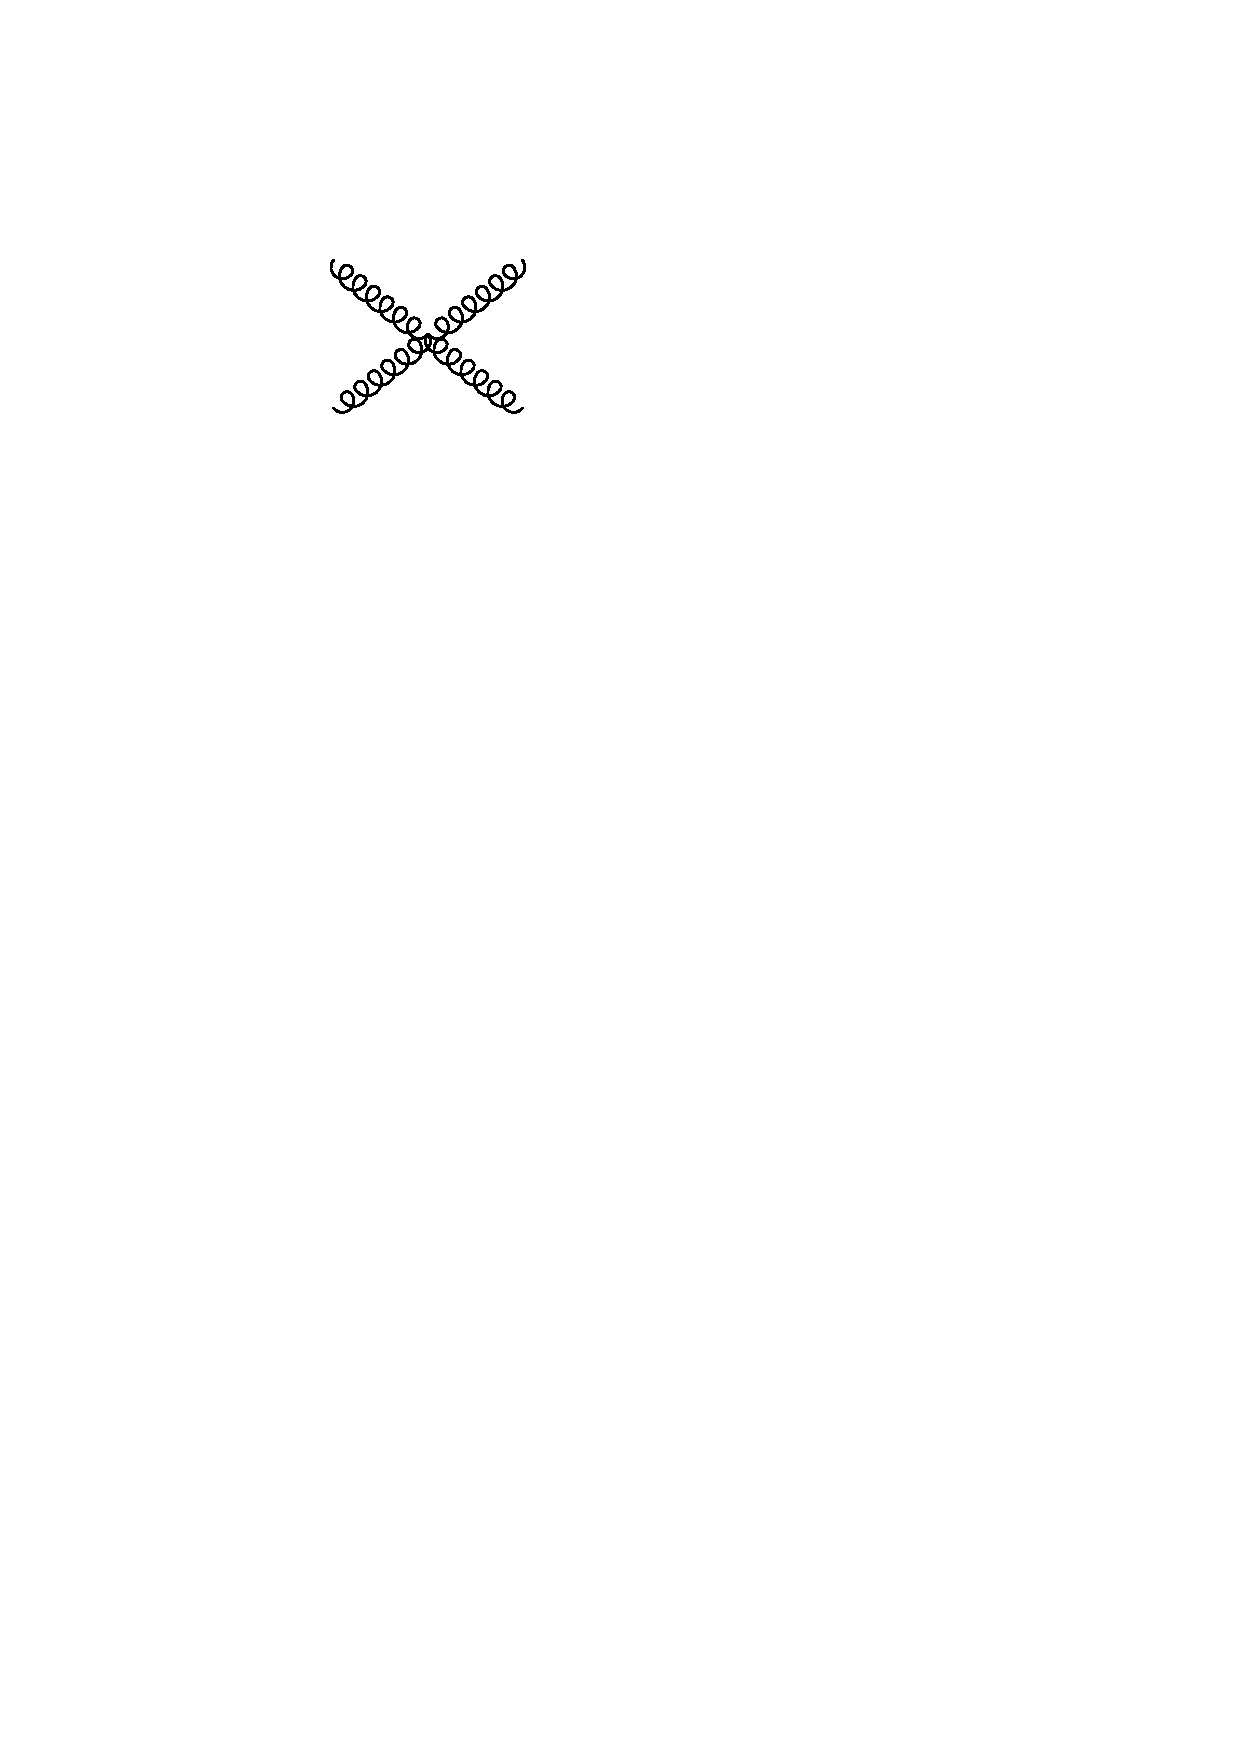
\includegraphics[width=0.3\textwidth]{fig/strongforce/gluon_four.pdf}
\end{center}
and the strength of the self-interaction is also characterised by $\alpha_s$. 
The self-interactions, together with the fact that $\alpha_s\sim 1$ means that the gluon field line density remains approximately constant with distance, in contrast to EM interactions where the field line density falls as $\frac{1}{r^2}$, as shown by the pictures below.
\begin{center}
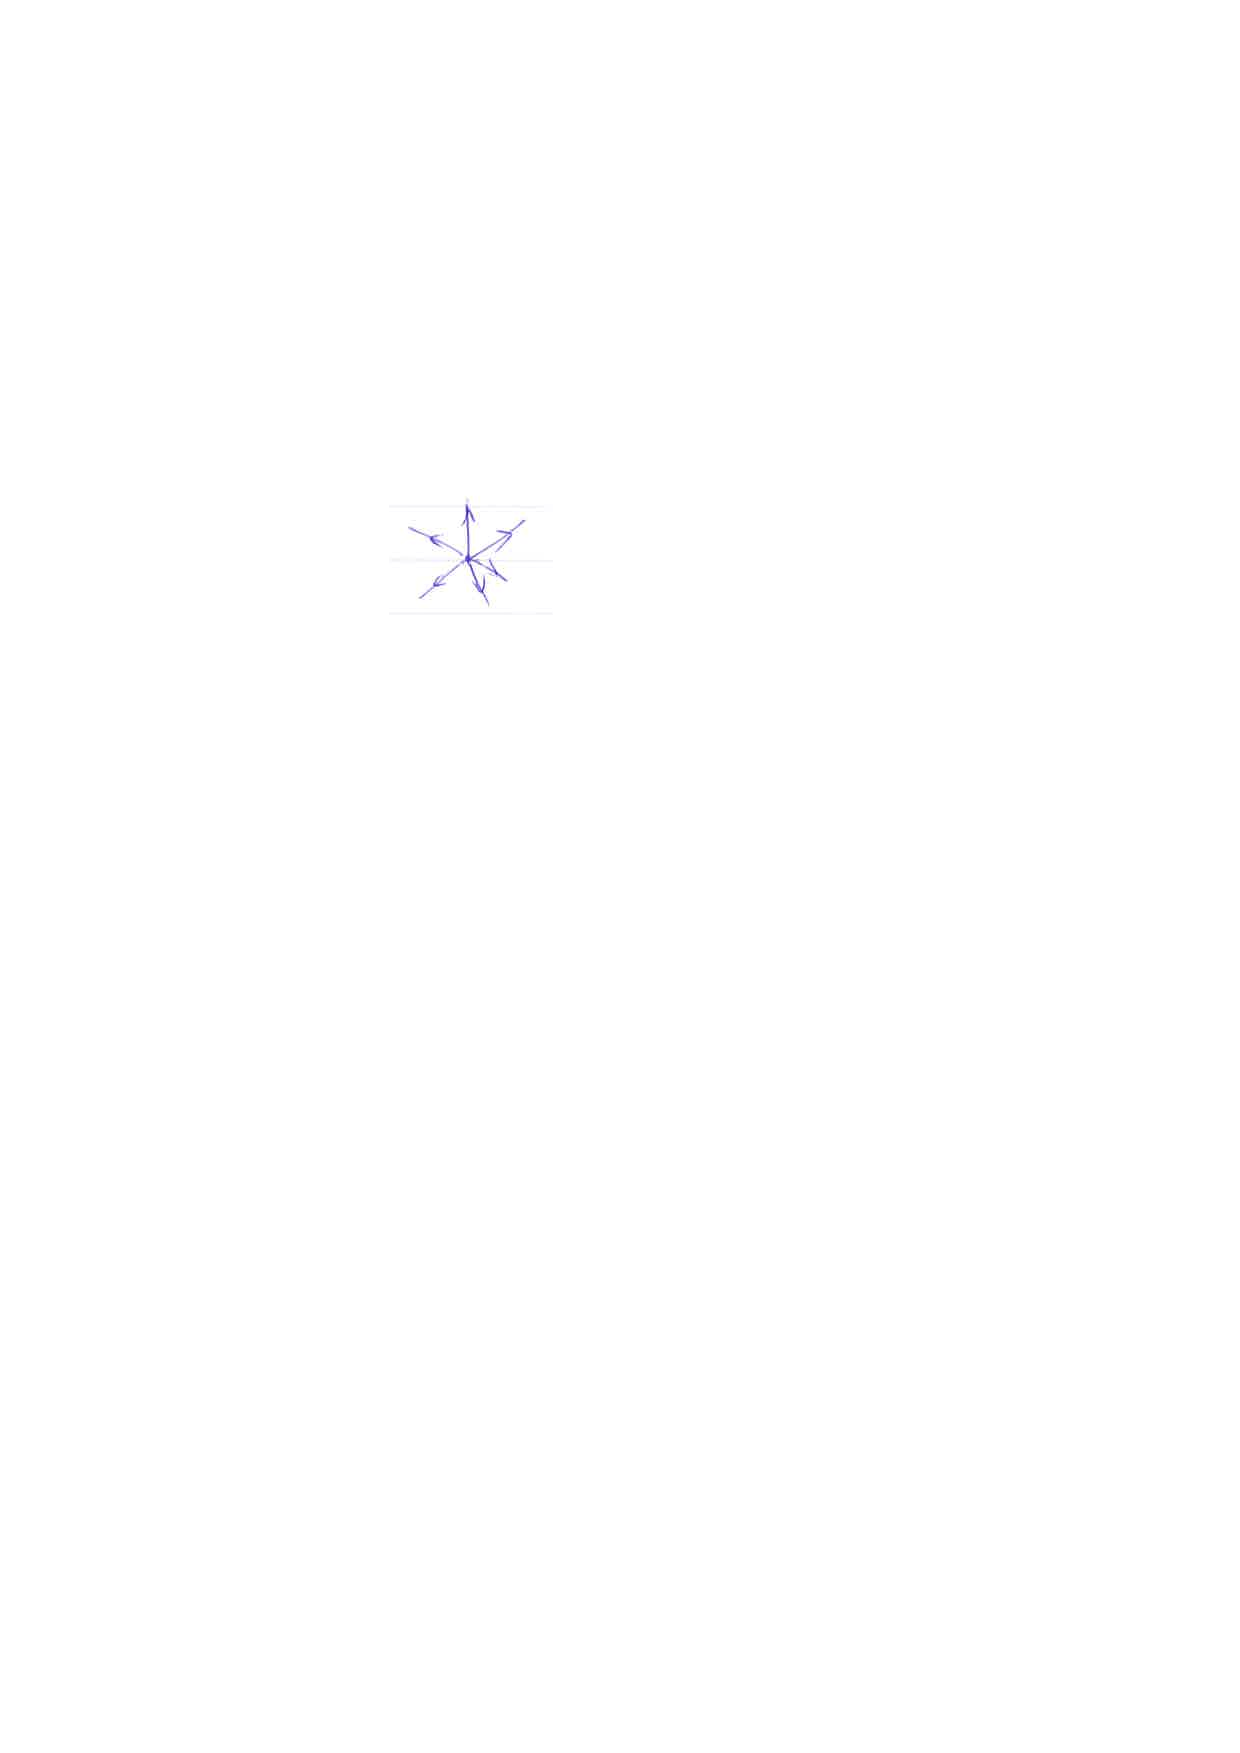
\includegraphics[width=0.3\textwidth]{fig/strongforce/em_line_density.pdf}
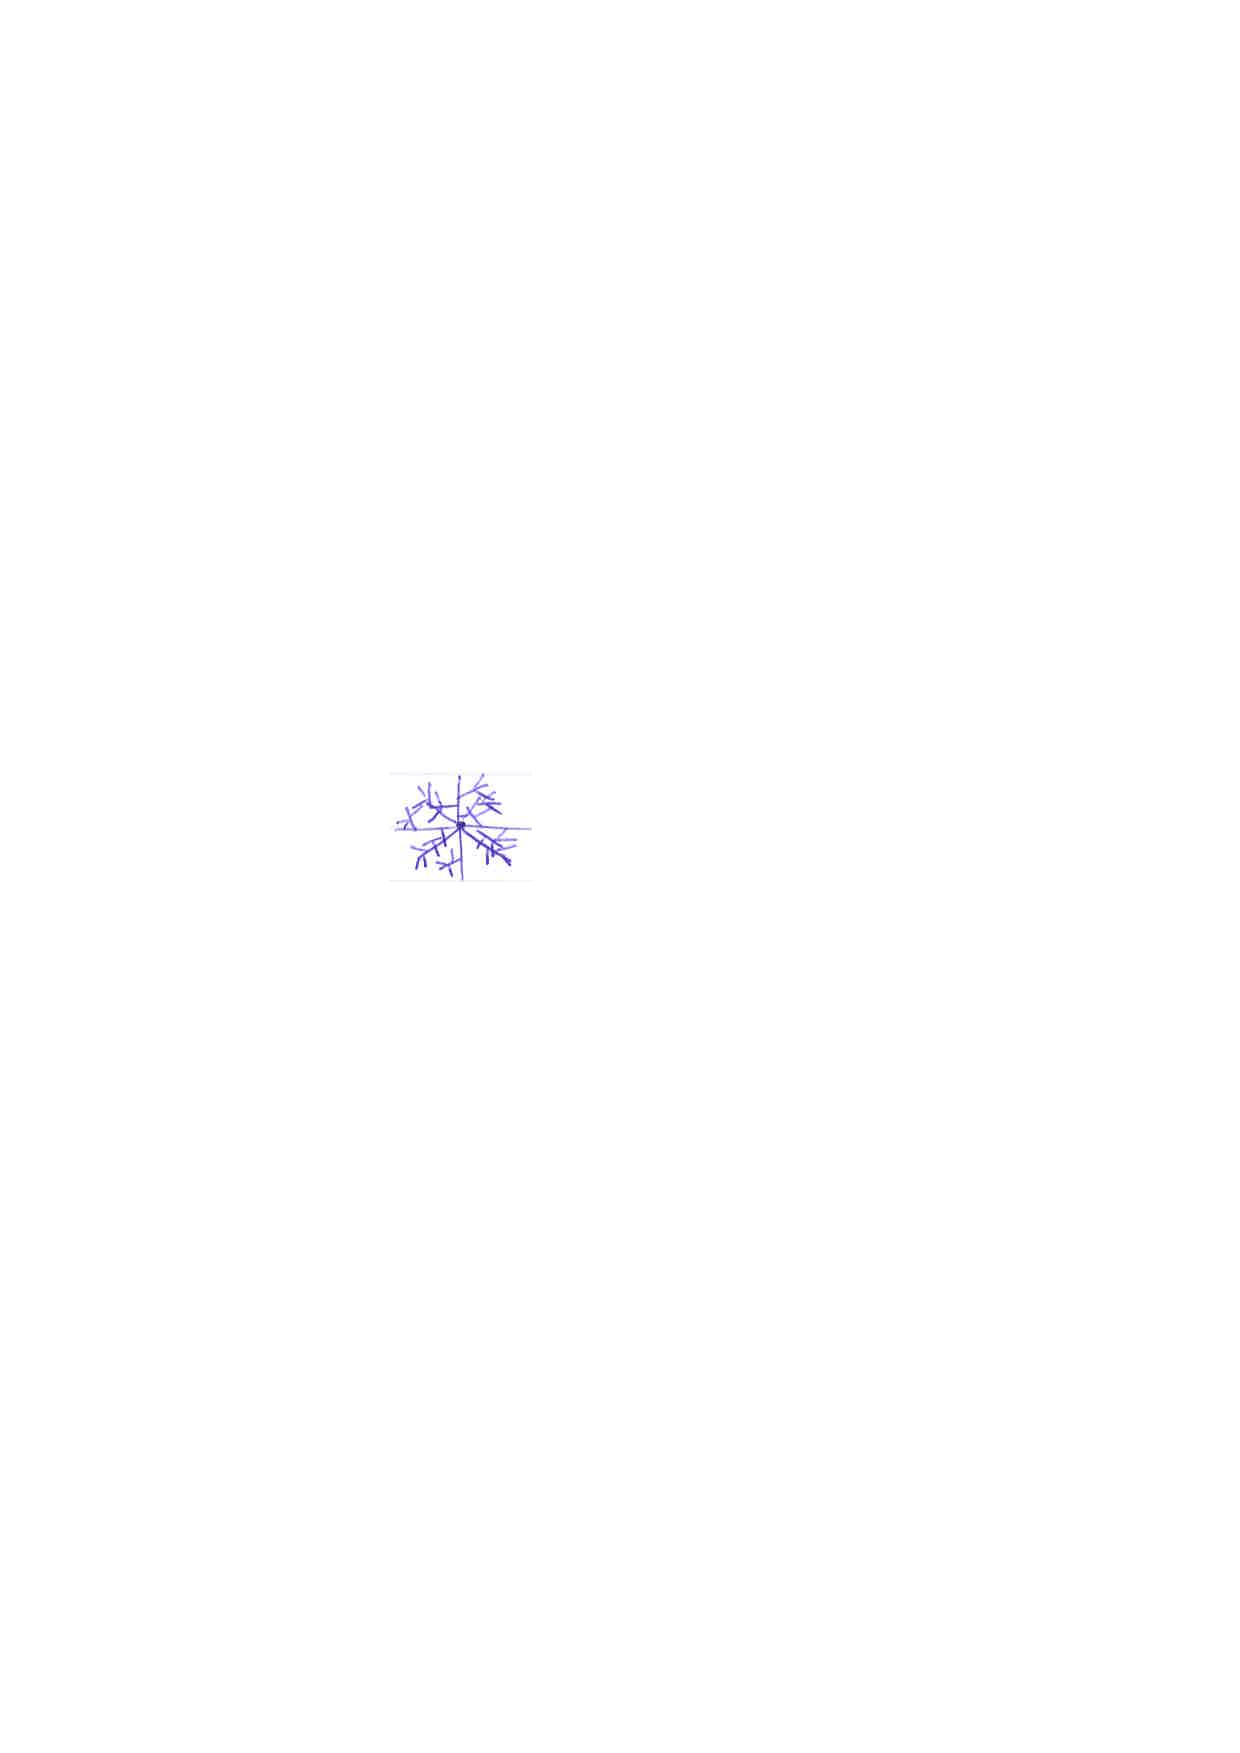
\includegraphics[width=0.3\textwidth]{fig/strongforce/strong_line_denstiy.pdf}\\
Pictures of EM field line density (left) and strong field line density (right)
\end{center}
So quarks can never be seen in complete isolation as they are constantly interacting with the field of the strong force. It takes around 1~GeV/fermi of energy to move a quark inside a hadron. As the masses of the up and down quarks are $\mathcal{O}(10)$~MeV, it is much more energetically favourable to produce quark-anti-quark pair which then forms a bound state rather than produce a free quark.

As it happens this is not the complete picture. As the energy (length)
scale of the strong process increases (decreases), the forces between
quarks becomes weaker. Therefore at large energies (small distances)
quarks can appear to move freely. This is why quarks within
hadrons appear to move freely within the hadron volume and the strong
coupling constant goes from $~1$ at an energy scale of 500~MeV to
$~0.1$ at 90~GeV. More information beyond the scope of the course can
be found in Appendix~\ref{sec:asymptotic_freedom}.

\subsection{Formation of jets}
\label{sec:FormationOfJets}
\begin{center}
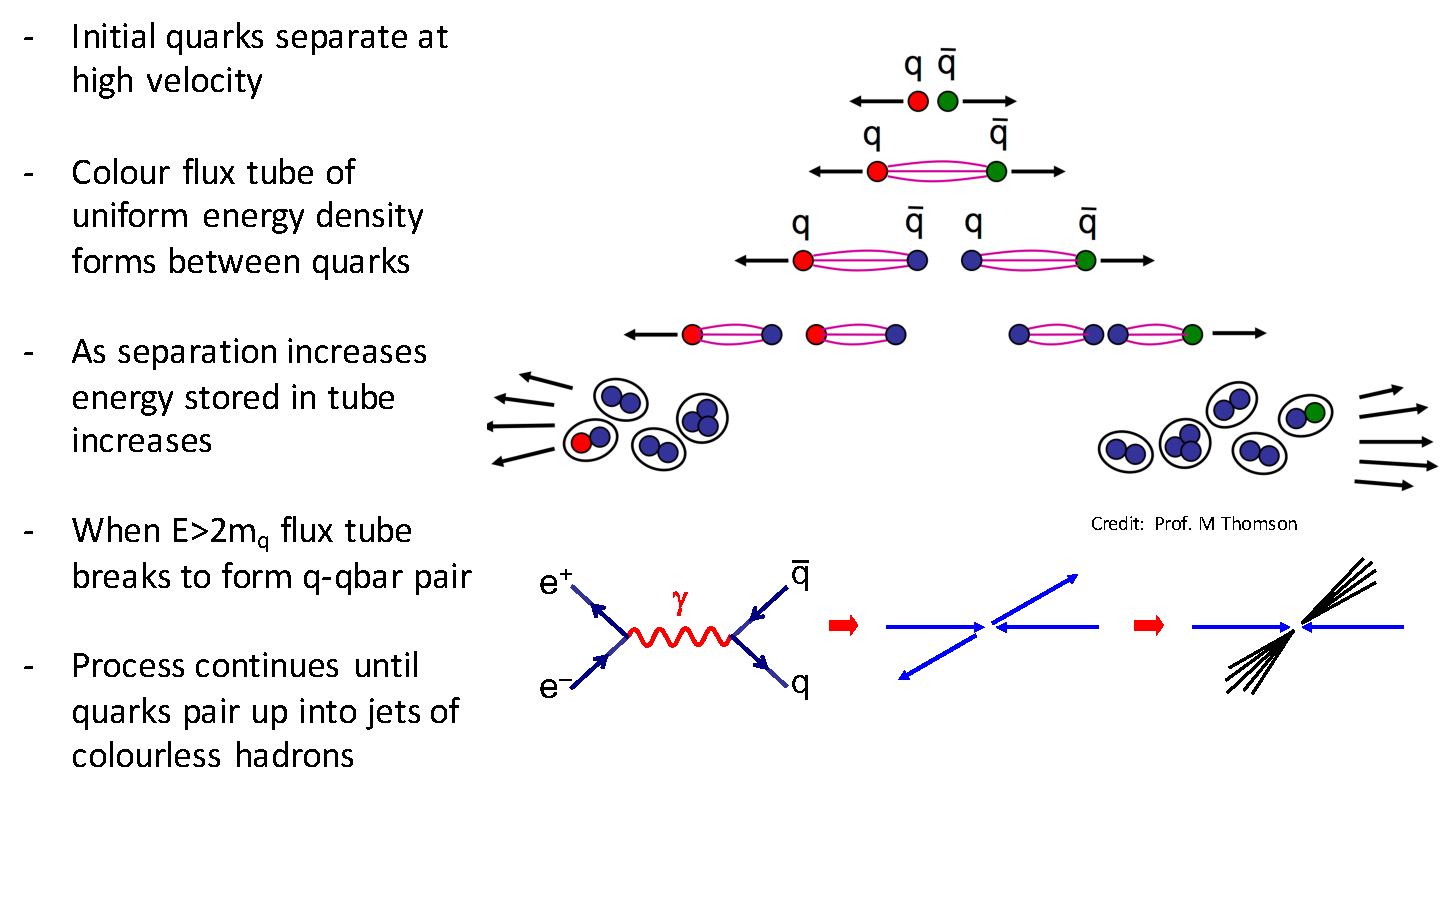
\includegraphics[width=0.97\textwidth]{fig/strongforce/jet_formation_2.pdf}
\end{center}

The picture below shows an example of a two-jet (di-jet) event produced from a collision of two protons at the LHC. 
\begin{center}
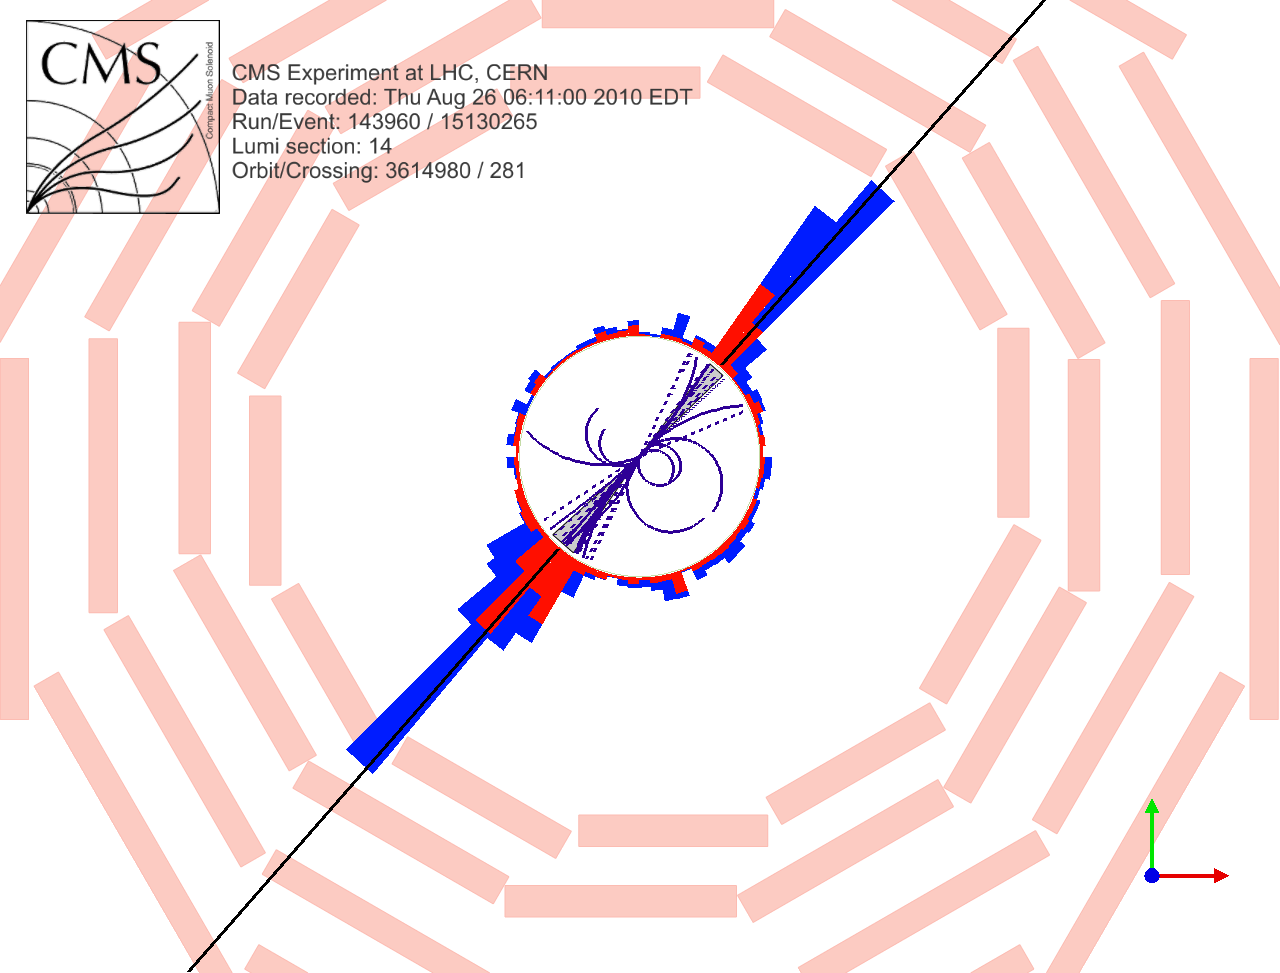
\includegraphics[width=0.4\textwidth]{fig/strongforce/cms_dijet.png}
\end{center}


\paragraph{Further evidence for colour:}
As you saw last year, further evidence for the existence of colour-charge stems from the measurement of the $R$-ratio defined as:
\[
R=\frac{\sum_q\sigma(e^+e^-\to q\bar{q})}{\sigma(e^+e^-\to\mu^+\mu^-)}=3\times\sum_q e_{q}^{2}
\]
where the factor of 3 accounts for the fact that the quark-anti-quark pair can be produced in 3 states ($r\bar{r}$, $b\bar{b}$, $g\bar{g}$) and the sum runs over quark types and depends on the centre of mass energy of the collision. For example at LEP1 where $\sqrt{s}=91$~GeV, the sum runs up to and including the $b$-quark, however as the $t$-quark has a mass of $\sim 175$~GeV, there is not enough energy to produce a pair of them. So 
\[
R=3\times\left[\left(\frac{1}{3}\right)^2+\left(\frac{2}{3}\right)^2+\left(\frac{1}{3}\right)^2+\left(\frac{2}{3}\right)^2+\left(\frac{1}{3}\right)^2\right]=\frac{11}{3}
\]
which agrees well with experimental measurements. If colour charge did not exist then the $R$ ratio should have been $\frac{11}{9}$.

\paragraph{Further evidence for the gluon:}
Further evidence for the existence of the gluon stems from the observation of events containing three jets. These could only have occurred if the final state of the interaction contained a quark, an anti-quark and a gluon, each individually resulting in a jet.
\begin{center}
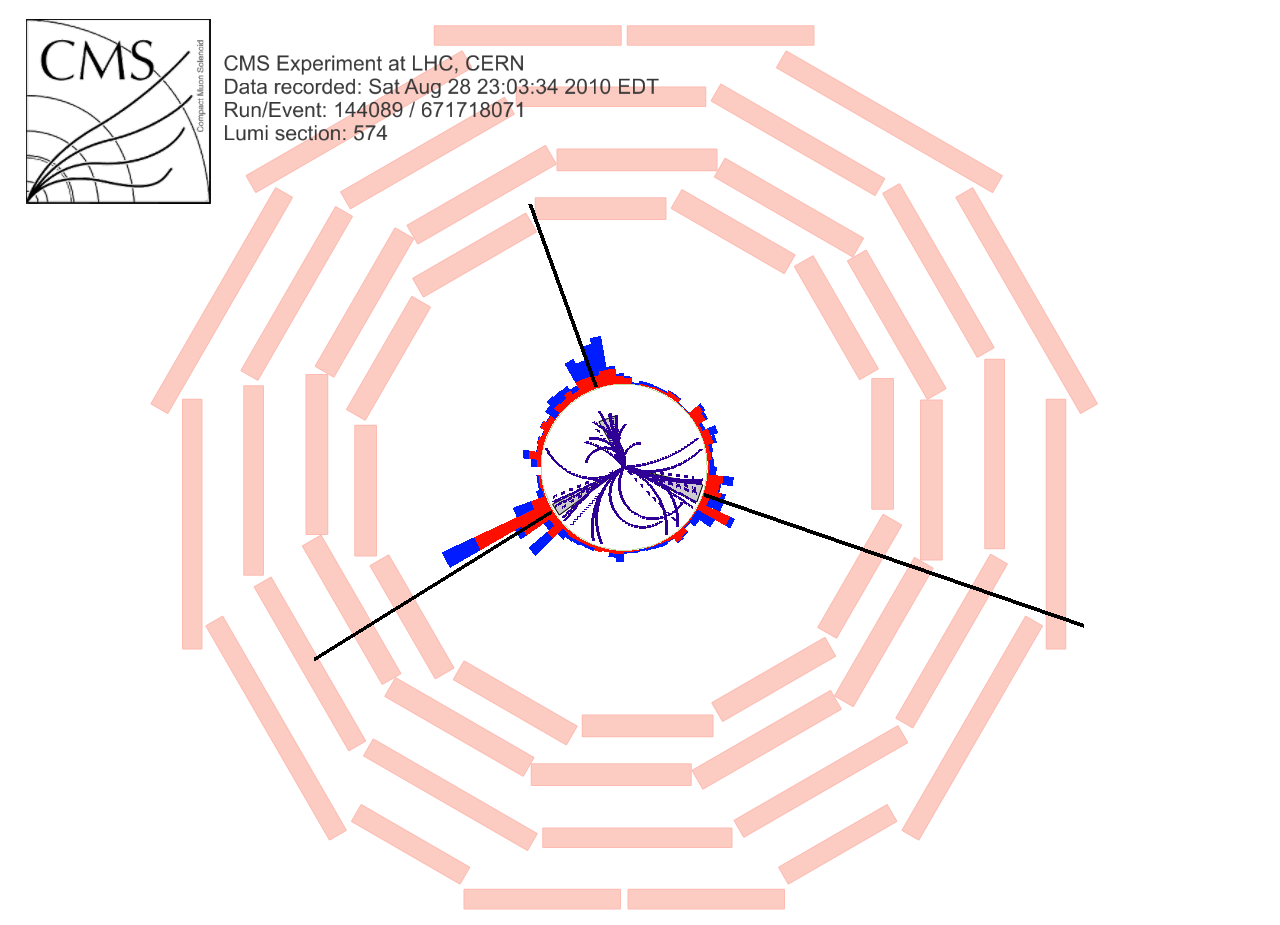
\includegraphics[width=0.5\textwidth]{fig/strongforce/cms_trijet.png}
\end{center}




